\documentclass[twoside,times]{article}
\usepackage[accepted]{aistats2e}

\usepackage{times}
\usepackage{subfigure}
\usepackage{amsmath}
\usepackage{bm}
\usepackage{bbm}
\usepackage{amsfonts}
\usepackage{amssymb}
\usepackage{graphicx}
\usepackage{natbib}
\usepackage{color}

\newcommand{\neil}[1]{\textbf{\textcolor{red}{Neil: #1}}}
%%%%%%%%%%%%%%%%%%%%%%%%%%%%%%%%%%%%%%%%%%%%%%%%%%%%%%%%%%%%%%%%%%%%
%
%  Utilities for typesetting in latex
%
%  Chris Williams, 1997, modified from utils.tex belonging to
%  Chris Bishop, 4 June 1995.
%
%
%%%%%%%%%%%%%%%%%%%%%%%%%%%%%%%%%%%%%%%%%%%%%%%%%%%%%%%%%%%%%%%%%%%%

\newcommand{\be}{\begin{equation}}
\newcommand{\ee}{\end{equation}}
\newcommand{\bi}{\begin{itemize}}
\newcommand{\ei}{\end{itemize}}
\newcommand{\bea}{\begin{eqnarray}}
\newcommand{\eea}{\end{eqnarray}}
\newcommand{\HOME}{/user/cs_neural/willicki}
%\newcommand{\COREL}{/user/cs_neural/bishopc/corel}

\newcommand{\bfdelta}{\boldsymbol{\delta}}
\newcommand{\bfDelta}{\boldsymbol{\Delta}}
\newcommand{\bfbeta}{\boldsymbol{\beta}}
\newcommand{\bfgamma}{\boldsymbol{\gamma}}
\newcommand{\bfmu}{\bm{\mu}}
%\newcommand{\bfmu}{\boldsymbol{\mu}}
\newcommand{\bfnu}{\boldsymbol{\nu}}
\newcommand{\bfalpha}{\boldsymbol{\alpha}}
\newcommand{\bfepsilon}{\boldsymbol{\epsilon}}
\newcommand{\bfSigma}{\boldsymbol{\Sigma}}
\newcommand{\bftau}{\boldsymbol{\tau}}
\newcommand{\bflambda}{\boldsymbol{\lambda}}
\newcommand{\bfLambda}{\boldsymbol{\Lambda}}
\newcommand{\bfpsi}{\boldsymbol{\psi}}
\newcommand{\bfxi}{\boldsymbol{\xi}}
\newcommand{\bfpi}{\bm{\pi}}
%\newcommand{\bfpi}{\boldsymbol{\pi}}
\newcommand{\bfPsi}{\boldsymbol{\Psi}}
\newcommand{\bfphi}{\boldsymbol{\phi}}
\newcommand{\bfPhi}{\boldsymbol{\Phi}}
\newcommand{\bfrho}{\boldsymbol{\rho}}
\newcommand{\bftheta}{\boldsymbol{\theta}}
\newcommand{\bfTheta}{\boldsymbol{\Theta}}
\newcommand{\bfomega}{\boldsymbol{\omega}}

\newcommand{\Bmath}[1]{\boldsymbol{#1}}

\newcommand{\bfa}{\mathbf{a}}
\newcommand{\bfb}{\mathbf{b}}
\newcommand{\bfc}{\mathbf{c}}
\newcommand{\bfd}{\mathbf{d}}
\newcommand{\bfe}{\mathbf{e}}
\newcommand{\bff}{\mathbf{f}}
\newcommand{\bfg}{\mathbf{g}}
\newcommand{\bfh}{\mathbf{h}}
\newcommand{\bfk}{\mathbf{k}}
\newcommand{\bfl}{\mathbf{l}}
\newcommand{\bfm}{\mathbf{m}}
\newcommand{\bfn}{\mathbf{n}}
\newcommand{\bfo}{\mathbf{o}}
\newcommand{\bfp}{\mathbf{p}}
\newcommand{\bfq}{\mathbf{q}}
\newcommand{\bfr}{\mathbf{r}}
\newcommand{\bfs}{\mathbf{s}}
\newcommand{\bft}{\mathbf{t}}
\newcommand{\bfu}{\mathbf{u}}
\newcommand{\bfv}{\mathbf{v}}
\newcommand{\bfw}{\mathbf{w}}
\newcommand{\bfx}{\mathbf{x}}
\newcommand{\bfy}{\mathbf{y}}
\newcommand{\bfz}{\mathbf{z}}

\newcommand{\bfzero}{\mathbf{0}}
\newcommand{\bfone}{\mathbf{1}}

\newcommand{\bfA}{\mathbf{A}}
\newcommand{\bfB}{\mathbf{B}}
\newcommand{\bfC}{\mathbf{C}}
\newcommand{\bfD}{\mathbf{D}}
\newcommand{\bfE}{\mathbf{E}}
\newcommand{\bfG}{\mathbf{G}}
\newcommand{\bfH}{\mathbf{H}}
\newcommand{\bfI}{\mathbf{I}}
\newcommand{\bfK}{\mathbf{K}}
\newcommand{\bfL}{\mathbf{L}}
\newcommand{\bfM}{\mathbf{M}}
\newcommand{\bfO}{\mathbf{O}}
\newcommand{\bfP}{\mathbf{P}}
\newcommand{\bfQ}{\mathbf{Q}}
\newcommand{\bfR}{\mathbf{R}}
\newcommand{\bfS}{\mathbf{S}}
\newcommand{\bfT}{\mathbf{T}}
\newcommand{\bfU}{\mathbf{U}}
\newcommand{\bfV}{\mathbf{V}}
\newcommand{\bfW}{\mathbf{W}}
\newcommand{\bfX}{\mathbf{X}}
\newcommand{\bfY}{\mathbf{Y}}
\newcommand{\bfZ}{\mathbf{Z}}
\newcommand{\llangle}{{\langle \vspace{-2mm} \langle}}
\newcommand{\rrangle}{{\rangle \vspace{-2mm} \rangle}}
\newcommand{\la}{\leftarrow}

\newcommand{\tf}{\tilde{f}}
\newcommand{\tg}{\tilde{g}}
\newcommand{\tX}{\tilde{X}}
\newcommand{\tY}{\tilde{Y}}
\newcommand{\tZ}{\tilde{Z}}

\newcommand{\bbE}{\mathbb{E}}
\newcommand{\bbR}{\mathbb{R}}
\newcommand{\bbP}{\mathbb{P}}
\newcommand{\bbT}{\mathbb{T}}
\newcommand{\bbZ}{\mathbb{Z}}

% for Fourier analysis
\newcommand{\ois}{2 \pi i s}  % ois is mnemonic for omega i of s
\newcommand{\oik}{2 \pi i k}  % ois is mnemonic for omega i of k
\newcommand{\oin}{2 \pi i n}  % ois is mnemonic for omega i of n
\newcommand{\oim}{2 \pi i m}  % ois is mnemonic for omega i of m

%\newcommand{\T}{\mathop{\rm T}\nolimits}
\newcommand{\T}{{\rm T}}
%\newcommand{\iint}{\int \! \! \int}
%\newcommand{\iiint}{\int \! \! \int \! \! \int}
\newcommand{\Tr}{\mbox{Tr}}
\newcommand{\diff}[1]{{\,d#1}}
\newcommand{\vgraph}[1]{
  \newpage
  \begin{center}
  {\large \bf #1}
  \end{center}
  \vspace{2mm}
}
%%\newcommand{\lapproxeq}{\stackrel{\textstyle <}{\sim}}
\newcommand{\high}[1]{\textcolor{blue}{\emph{#1}}}
\newcommand{\cut}[1]{}
\newcommand{\citeasnoun}[1]{\citeN{#1}}
\newcommand{\citemulti}[2]{(#1, \citeyearNP{#2})}
\newcommand{\citemultiN}[2]{#1 (\citeyearNP{#2})}
\newcommand{\Sum}{{\displaystyle \sum}}
\newcommand{\defeq}{{\stackrel{def}{=}}}
\newcommand{\marg}[1]{\marginpar{#1}}

%%%%%%%%%%%%%%%%%%%%%%%%%%%%%%%%%%%%%%%%%%%%%%%%%%%%%%%%%%%%%%%%%%%%

\newcommand{\pdt}[2]{\frac{\partial^2 #1}{\partial {#2}^2 }}
\newcommand{\pdsd}[3]{\frac{\partial^2 #1}{\partial {#2} \partial {#3} }}
\newcommand{\pdo}[2]{\frac{\partial {#1}}{\partial {#2}}}
\newcommand{\pdol}[2]{\partial {#1}/ \partial {#2}}
\newcommand{\pdu}[1]{\frac{\partial }{\partial {#1}}}                          

%%% Local Variables: 
%%% mode: latex
%%% TeX-master: t
%%% End: 


% If your paper is accepted, change the options for the package aistats2e as follows
%\usepackage[accepted]{aistats2e}
% This option will print headings for the title of your paper and headings for the
% authors names, plus a copyright note at the end of the first column of the first page.


\begin{document}

\twocolumn[

\aistatstitle{Bayesian Gaussian Process Latent Variable Model}

\aistatsauthor{Michalis K. Titsias \And Neil D. Lawrence}

\aistatsaddress{ School of Computer Science\\ 
University of Manchester \And School of Computer Science\\ 
University of Manchester } ]

% Abstract

\begin{abstract}

  We introduce a variational inference framework for training 
  the Gaussian process latent variable model and thus performing 
  Bayesian nonlinear dimensionality reduction. This method allows us to variationally
  integrate out the input variables of the Gaussian process and
  compute a lower bound on the exact marginal likelihood of the
  nonlinear latent variable model. The maximization of the
  variational lower bound provides a Bayesian training procedure that is robust to
  overfitting and  can automatically select the dimensionality of the
  nonlinear latent space. We demonstrate our method on real world
  datasets. The focus in this paper is on dimensionality reduction
  problems, but the methodology is more general. For example, our
  algorithm is immediately applicable for training Gaussian process
  models in the presence of missing or uncertain inputs.

\end{abstract}

\section{Introduction}

Gaussian processes (GPs) \citep[see e.g.][]{Rasmussen:book06} are
stochastic processes over real-valued functions. GPs offer a Bayesian
nonparametric framework for inference of highly nonlinear latent
functions from observed data. They have become very popular in
machine learning for solving problems such as nonlinear regression
and classification.


The standard application of GP models is to supervised learning tasks
where both output and input data are assumed to be given at
training time. The application of GPs to unsupervised learning tasks
is more involved. One approach to unsupervised learning with GPs 
is the Gaussian process latent variable model (GP-LVM) proposed by
\cite{Lawrence:gplvm03,Lawrence:pnpca05}. GP-LVM can be considered as
a multiple-output GP regression model where only the output data are
given. The inputs are unobserved and are treated as latent
variables, however instead of integrating out the latent variables,
they are optimized. This trick makes the model tractable and some
theoretical grounding for the approach is given by the fact that the
model can be seen as a nonlinear extension of the linear
probabilistic PCA (PPCA). In PPCA (and in factor analysis (FA))
Bayesian extensions of the model are straightforward
\citep{Bishop:icann99,Ghahramani:bfa00} using variational algorithms
based on mean field approximations. An analogous variational method
for the GP-LVM is a much more challenging problem which had not been
addressed until this paper.  The main difficulty is that  to
apply variational Bayes to GP-LVM we need to approximately integrate
out the latent/input variables that appear nonlinearly in the inverse
kernel matrix of the GP model. Standard mean field variational
methodologies do not lead to an analytically tractable algorithm.

We introduce a framework that allows us to variationally
integrate out the latent variables in the GP-LVM and compute a
closed-form Jensen's lower bound on the true log marginal likelihood
of the data.  The key ingredient that makes the variational Bayes
approach tractable is the application of variational inference in an
\emph{expanded probability model} where the GP prior 
is augmented to include auxiliary inducing
variables. Inducing variables were introduced originally for
computational speed ups in GP regression models
\citep{Csato:sparse02,Seeger:fast03,Csato:thesis02,Snelson:pseudo05,Quinonero:unifying05,Titsias:variational09}. Our
approach builds on, and significantly extends the variational sparse
GP method of \citet{Titsias:variational09} so that a closed-form
variational lower bound of the GP-LVM marginal likelihood is
computed. This solves a key problem with the GP-LVM:  variational
inference in the GP-LVM allows for Bayesian training 
of the model that is robust to overfitting. Furthermore, by
using the automatic relevance determination (ARD) squared exponential
kernel, the algorithm allows us to automatically infer the dimensionality
of the nonlinear latent space without introducing explicit
regularizers to enforce this constraint \citep{Geiger:rank09}.

Although, in this paper, we focus on application of the variational
approach to the GP-LVM, the methodology we have developed can be more
widely applied to a variety of other GP models. In particular, our
algorithm is immediately applicable for training GPs with missing or
uncertain inputs \citep{Girard:uncertain01}. Other possible
applications will be discussed 
as future work.

In the remainder of the paper we first review the GP-LVM and then we
introduce our variational approximation. We finish by demonstrating
the ability of the new model to automatically determine dimensionality 
and resist overfitting on real world datasets. 

\section{Gaussian process latent variable model \label{sec:gplvm}}

Let $Y \in \mathbbm{R}^{N \times D}$ be the observed data where $N$ is
the number of observations and $D$ the dimensionality of each data
vector. These data are associated with latent variables $X \in
\mathbbm{R}^{N \times Q}$ where, for the purpose of doing
dimensionality reduction, $Q \ll D$.  The GP-LVM
\citep{Lawrence:pnpca05} defines a forward (or generative) mapping
from the latent space to observation space that is governed by
Gaussian processes. If the GPs are taken to be independent across the
features then the likelihood function is written as
\begin{equation}
p(Y|X) = \prod_{d=1}^D p(\bfy_d|X),
\label{eq:GP-LVMlikel}
\end{equation} 
where $\bfy_d$ represents the $d^{\text{th}}$ column of $Y$ and 
\begin{equation}
p(\bfy_d|X) = \mathcal{N}(\bfy_d|\bfzero, K_{NN} + \beta^{-1} I_N).
\end{equation}         
Here, $K_{NN}$ is the $N \times N$ covariance matrix defined by the covariance (or kernel)
function $k(\bfx,\bfx')$. For the purpose of doing automatic model
selection of the dimensionality of latent space, this kernel can
be chosen to follow the ARD \citep[see][]{Rasmussen:book06} squared
exponential form:
\begin{equation}
k(\bfx,\bfx') = \sigma_f^2 \exp\left( - \frac{1}{2} \sum_{q=1}^Q
\alpha_q (x_q - x_q')^2 \right). 
\label{eq:ARDkernel}
\end{equation} 
Equation (\ref{eq:GP-LVMlikel}) can be viewed as the likelihood
function of a multiple-output GP regression model where the vectors of
different outputs are drawn independently from the same Gaussian
process prior which is evaluated at the inputs $X$.  Since $X$ is a
latent variable, we can assign it a prior density given by the
standard normal density. % in a manner analogous to FA and PPCA models. 
More precisely, the prior for $X$ is:
\begin{equation} 
p(X) = \prod_{n=1}^N \mathcal{N}(\bfx_n|\bfzero,I_Q), 
\end{equation}
where each $\bfx_n$ is the $n^{\text{th}}$ row of $X$.
The joint probability model for the GP-LVM model is 
\begin{equation}
p(Y,X) = p(Y|X) p(X).
\end{equation}
The hyperparameters of the model are the kernel parameters $\bftheta =
(\sigma_f^2, \alpha_1,\ldots,\alpha_Q)$
and the inverse variance parameter $\beta$.  For the sake of clarity,
these parameters are omitted from the conditioning of the
distribution\footnote{A precise notation is to write
  $p(Y,X|\beta,\bftheta) = p(Y|X,\beta,\bftheta) p(X)$.}.  Currently,
the primary methodology for training the GP-LVM model is to find the
MAP estimate of $X$ \citep{Lawrence:pnpca05} whilst jointly maximizing
with respect to the hyperparameters. Here, we develop a variational
Bayesian approach to marginalization of the latent variables, $X$,
allowing us to optimize the resulting lower bound on the marginal
likelihood with respect to the hyperparameters. The lower bound can
also be used for model comparison and automatic selection of the latent
dimensionality.

\section{Variational inference \label{sec:varInf}} 

We wish to compute the marginal likelihood of the data:
\begin{equation}
p(Y) =  \int p(Y|X) p(X) d X.
\end{equation}    
However, this quantity is intractable as $X$ appears nonlinearly
inside the inverse of the covariance matrix $K_{NN} + \beta^{-1}I_N$. Instead, we seek to
apply an approximate variational inference procedure where we
introduce a variational distribution $q(X)$ to approximate the true
posterior distribution $p(X|Y)$ over the latent variables.  We take
the variational distribution to have a factorized Gaussian form over
the latent variables,
\begin{equation}
q(X) = \prod_{n=1}^N \mathcal{N}(\bfx_n|\bfmu_n,S_n), 
\end{equation}
where the variational parameters are $\{\bfmu_n,S_n\}_{n=1}^N$ and,
for simplicity, $S_n$ is taken to be a diagonal covariance
matrix\footnote{This can be extended to non-diagonal within our
  framework.}. Using this variational distribution we can express a
Jensen's lower bound on the $\log p(Y)$ that takes the form:
\begin{align}
F(q) & = 
 \int q(X) \log \frac{p(Y|X)
  p(X)}{q(X)} d X \nonumber \\
 & =  \int q(X) \log p(Y|X) d X  
 - \int q(X) \log \frac{q(X)}{p(X)} d X  \nonumber \\ 
 & =  \widetilde{F} (q)   -  \text{KL}(q||p),
\label{eq:gplvmbound}
\end{align}
where the second term is the negative KL divergence between the
variational posterior distribution $q(X)$ and the prior distribution
$p(X)$ over the latent variables. This term is computed
analytically since both distributions are Gaussians. 
%; see eq.\ \label{eq:gplvmboundFinal} for an explicit expression. 
Therefore, the
difficult part when estimating the above bound is the first term:
\begin{equation} 
\widetilde{F} (q) = \sum_{d=1}^D \int q(X) \log p(\bfy_d|X) d X = \sum_{d=1}^D \widetilde{F}_d (q), 
\label{eq:fD}
\end{equation}  
%\neil{Here and later, why is $\widetilde{F}$ indexed by $n$ shouldn't it be $d$?}
where we have used (\ref{eq:GP-LVMlikel}). Thus, the computation of
$\widetilde{F} (q)$ breaks down to separate computations of each
$\widetilde{F}_d (q)$, corresponding to the $d^{\text{th}}$ output.  Notice that
the computation of $\widetilde{F}_d (q)$ involves an analytically
intractable integration. This arises because $\log p(\bfy_d|X)$
contains $X$ in an highly nonlinear manner inside the inverse of
the covariance matrix, $K_{NN} + \beta^{-1} I_N$. Our main contribution
is a mathematical tool that allows us to compute a closed-form lower
bound for $\widetilde{F}_d (q)$. As we will see, the key idea is to
apply variational sparse GP regression in an augmented probability
model.
%will aloow to compute the above and efficiently optimize it over the
%variational distribution $q(X)$ and the model hyperparameters 
%$(\beta,\bftheta)$. 


\subsection{Lower bound  by applying
 variational sparse GP regression}

The computation in $\widetilde{F}_d (q)$ involves an
expectation over the intractable term 
$\log p(\bfy_d |X)$. To deal with this, we first compute a Jensen's
lower bound on $\log p(\bfy_d| X)$ by introducing the GP latent
function values together with auxiliary inducing variables as those
used in sparse GP models. 

Sparse approximations have already been applied to speed up the GP-LVM
\cite{Lawrence:larger07}. The first step of our approximation is
equivalent to applying the new variational approximation of
\citet{Titsias:variational09} to the standard GP-LVM. The likelihood
function $p(\bfy_d|X)$ is just the Gaussian marginal likelihood of a
GP regression model. We % can 
make this explicit by introducing the GP
latent function values $\bff_{d} \in \mathbbm{R}^N$ associated with
the vector of (noise corrupted) outputs $\bfy_d$ (the $d^{\text{th}}$ column of
$Y$). The ``complete'' likelihood % function 
associated with the
marginal likelihood $p(\bfy_d|X)$ is:
\begin{equation}
p(\bfy_d,\bff_d|X) = p(\bfy_d|\bff_d)
p(\bff_d|X),
\label{eq:jointmodelwithlatent}
\end{equation}     
where $p(\bfy_d|\bff_d) = \mathcal{N}(\bfy_d | \bff_d, \beta^{-1} I_N)$ and
$p(\bff_d|X)$ is the zero-mean GP prior with covariance matrix
$K_{NN}$. Note that the above joint % probability 
model still contains
$X$ inside the inverse of $K_{NN}$ making expectations under
distributions over $X$ difficult to compute. We finesse this
intractability by introducing auxiliary inducing variables and
applying the variational sparse GP formulation of
\citet{Titsias:variational09}.
 
We follow the approach of \citet{Lawrence:larger07}: for each vector
of latent function values $\bff_d$ we introduce a separate set of $M$
inducing variables $\bfu_d \in \mathbbm{R}^M$ evaluated at a set of inducing input
locations given by $Z \in \mathbbm{R}^{M \times Q}$. For simplicity, we assume that all $\bfu_d$s,
associated with different outputs, are evaluated at the same inducing
locations, %$Z = (\bfz_1,\ldots, \bfz_M)$, 
however this could be relaxed. The $\bfu_d$ variables are just function points drawn from
the GP prior. Using these inducing variables we augment the joint
probability model in eq.\ (\ref{eq:jointmodelwithlatent}):
\begin{equation}
p(\bfy_d,\bff_d,\bfu_d|X,Z) = p(\bfy_d|\bff_d)
p(\bff_d|\bfu_d, X, Z) p(\bfu_d | Z), 
\label{eq:jointmodelwithlatentandInd}
\end{equation}      
where we used the fact that the joint GP prior over function values
$\bff_d$ and $\bfu_d$ evaluated at inputs $X$ and $Z$ %respectively
factorizes as $p(\bff_d,\bfu_d|X, Z) = p(\bff_d|\bfu_d, X, Z) p(\bfu_d
| Z)$ where
$$
p(\bff_d|\bfu_d, X, Z) = \mathcal{N}(\bff_d |\bfalpha_d, 
K_{NN} - K_{NM} K_{MM}^{-1} K_{MN})
$$ 
is the conditional GP prior with $\bfalpha_d = K_{NM} K_{MM}^{-1} \bfu_d$. 
Further, $p(\bfu_d|Z) = \mathcal{N}(\bfu_d | \bfzero, K_{MM})$ is the
marginal GP prior over the inducing variables. The likelihood $p(\bfy_d |
X)$ can be equivalently computed from the above augmented model by
marginalizing out $(\bff_d, \bfu_d)$ and crucially this is true for
any value of the inducing inputs $Z$. This means that, unlike $X$, the
inducing inputs $Z$ are \emph{not} random variables. Neither are they
model hyperparameters, %as $(\bftheta,\beta)$ 
they are \emph{variational parameters}. This interpretation of the inducing
inputs is key in developing our approximation, it arises from the
variational approach of \citet{Titsias:variational09}.  Taking
advantage of this observation we now simplify our expressions by dropping
$Z$ from our notation. We can now apply variational inference to
approximate the true posterior,
$
p(\bff_d,\bfu_d|\bfy_d,X) = p(\bff_d |\bfu_d, \bfy_d, X) p(\bfu_d|\bfy_d, X), 
$
with a sparse variational distribution that takes the form  
%Crucially this will allow 
%to obtain a lower bound for the log
%likelihood $\log p(Y|X)$ that will be amenable to tractable computations. 
%Therefore, we introduce the variational distribution: 
\begin{equation}
q(\bff_d,\bfu_d) =  p(\bff_d|\bfu_d,X) \phi(\bfu_d),
\end{equation} 
where $p(\bff_d|\bfu_d,X)$ is the conditional GP prior that 
appears in the joint model in
(\ref{eq:jointmodelwithlatentandInd}), while $\phi(\bfu_d)$ is a
variational distribution over the inducing variables $\bfu_d$. 
Thus we obtain a lower bound: 
\begin{multline}
\log p(\bfy_d | X) 
\geq  \int \phi(\bfu_d) 
\log \frac{ p(\bfu_d) \mathcal{N}(\bfy_d| \bfalpha_d,
\beta^{-1} I_N) }{\phi(\bfu_d)} d \bfu_d \\
- \frac{\beta}{2} 
\text{Tr} (K_{NN} - K_{NM} K_{MM}^{-1} K_{MN}), 
\label{eq:lowerboundofF1}
\end{multline} 
%where $\phi(U) = \prod_{d=1}^D \phi(\bfu_d)$ and $p(U) = \prod_{d=1}^D
% p(\bfu_d|Z)$.  
where $\bfalpha_d =  K_{NM} K_{MM}^{-1} \bfu_d$. 
In the variational sparse GP method \citep{Titsias:variational09}, 
the $\phi(\bfu_d)$ distribution is computed in an optimal way. 
Such an optimal choice of this distribution depends on
the latent variables $X$ and is not useful in our case. In order 
to obtain the bound for the GP-LVM we need to take a mean field
approach and force independence of the
%variational
distribution  
$\phi(\bfu_d)$ from the random variable $X$. 


% \subsection{The variational lower  bound}   

% Recall that our goal in this section is to approximate 
% $\widetilde{F}_n (q)$ in eq.\ (\ref{eq:f1}) with a variariatinal 
% lower bound. 
So far we have computed a lower bound on $\log p(\bfy_d | X)$ which is
the intractable term in $\widetilde{F}_d (q)$. Using eq.\ 
(\ref{eq:lowerboundofF1}) and the definition of $\widetilde{F}_d (q)$
from (\ref{eq:fD}) we have
%
%In the previous section we provided  a variational lower bound for the
%the log likelihood $\log p(X|Y)$ by applying variational sparse GP regression
%using auxiliary inducing variables. Assuming now that
%$U$ and  $X$ are independent in the underlying variational approximate 
%posterior, we can compute analytically a lower bound of $F_1(q)$.
%More precisely, the $F_1(q)$ term  is approximated by a Jensen's 
%lower bound: 
\begin{align*}
\widetilde{F}_d(q) & \geq 
\int q(X) \Bigl[  \int \phi(\bfu_d)
\log \frac{p(\bfu_d) \mathcal{N}(\bfy_d|\bfalpha_d, \beta^{-1} I_N)}
{\phi(\bfu_d)} d \bfu_d \Bigl. \nonumber \\ 
& \Bigr. - \frac{\beta}{2} \text{Tr} (K_{NN})  +  \frac{\beta}{2} \text{Tr} (K_{MM}^{-1}
K_{MN} K_{NM})  \Bigr] d X,   
\end{align*}
where we used standard properties of the  trace of a matrix.
%where we substituted the r.h.s.\  expression of eq.\
%(\ref{eq:lowerboundofF1})  into eq.\ (\ref{eq:f1}). 
Since (under our factorization assumption) $\phi(\bfu_d)$ does not
depend on the random variable $X$, we can swap the integrations over
$X$ and $\bfu_d$ and perform firstly the integration with respect to
$X$:
\begin{align*} 
& \widetilde{F}_d(q)  \geq \\
& \int \phi(\bfu_d)  \left[
 \langle \log \mathcal{N}(\bfy_d| \bfalpha_d, \beta^{-1} I_N) \rangle_{q(X)} + 
  \log \frac{p(\bfu_d)}{\phi(\bfu_d)} 
\right] d \bfu_d \\ 
& -  
 \frac{\beta}{2} \text{Tr} \left( \langle K_{NN} \rangle_{q(X)} \right)
+ \frac{\beta}{2} \text{Tr} \left( K_{MM}^{-1} \langle K_{MN}
K_{NM} \rangle_{q(X)} \right),    
\end{align*}
where $\langle \cdot \rangle_{q(X)}$ denotes expectation under the
distribution $q(X)$.  Now, we can analytically
maximize the above lower bound with respect to the distribution
$\phi(\bfu_d)$. The optimal setting of this distribution is 
$\phi (\bfu_d) \propto \langle \log \mathcal{N}(\bfy_d| \bfalpha_d, \beta^{-1} I_N)
\rangle_{q(X)} p(\bfu_d)$ and the lower bound that automatically incorporates
such an optimal setting is obtained easily by reversing Jensen's inequality,
\begin{multline}
\widetilde{F}_d(q) 
\geq  \log \left( \int e^{ \langle \log \mathcal{N}(\bfy_d| \bfalpha_d,
\beta^{-1} I_N) \rangle_{q(X)}} p(\bfu_d) d \bfu_d \right) \\
- \frac{\beta }{2} \text{Tr} \left( \langle K_{NN} \rangle_{q(X)} \right)
+ \frac{\beta }{2}  \text{Tr} \left( K_{MM}^{-1} \langle K_{MN}
K_{NM} \rangle_{q(X)} \right) \nonumber.    
%\label{eq:tildef1}
\end{multline}
The r.h.s.\ in this equation is a lower bound in which the
variational distribution $\phi(\bfu_d)$ has been 
eliminated optimally.   
This quantity now can be computed in closed-form since it boils down
to computing the statistics $\psi_0 = \text{Tr} \left( \langle K_{NN}
\rangle_{q(X)} \right)$, $\Psi_1 = \langle K_{NM} \rangle_{q(X)}$
and $\Psi_2 = \langle K_{MN} K_{NM} \rangle_{q(X)}$. These statistics
for certain covariance functions, such as the ARD squared exponential
from (\ref{eq:ARDkernel}), are computable analytically as discussed in
section \ref{sec:psiStats}. Notice also that $\langle \log \mathcal{N}(\bfy_d|
\bfalpha_d, \beta^{-1} I_N) \rangle_{q(X)}$ is just a quadratic function
of $\bfu_d$ that depends on the statistics $\Psi_1$ and
$\Psi_2$. Therefore, the integration involved in the above equation is
a standard Gaussian integral. The closed-form of the lower bound on 
$\widetilde{F}_d(q)$ is:
\begin{align}
\widetilde{F}_d(q) & \geq \log \left[ \frac{(\beta)^{\frac{N}{2}} |K_{MM}|^{\frac{1}{2}}}
{(2 \pi)^{\frac{N}{2}}|\beta \Psi_2 + K_{MM}|^{\frac{1}{2}}} 
e^{ - \frac{1}{2} \bfy_d^T W \bfy_d} \right] \nonumber \\
&  -  \frac{\beta \psi_0}{2}  +  
\frac{\beta}{2} \text{Tr} \left(K_{MM}^{-1} \Psi_2 \right),
\label{eq:Fdbound}
\end{align}
where $W = \beta I_N  -  \beta^2 \Psi_1 (
\beta \Psi_2 + K_{MM})^{-1} \Psi_1^T$. We can now compute the
closed-from variational lower of the GP-LVM 
according to equation (\ref{eq:gplvmbound}). More precisely, by
summing both sides of (\ref{eq:Fdbound}) over the $D$ outputs 
we obtain on the l.h.s.\ the term $\widetilde{F}(q)$ (see equation
(\ref{eq:fD})) and on the r.h.s.\ a lower bound on  
$\widetilde{F}(q)$. By substituting the latter quantity 
(in place of $\widetilde{F}(q)$) in (\ref{eq:gplvmbound}) 
we obtain the final GP-LVM lower bound.  
This bound has an elegant form since it resembles 
closely the corresponding sparse GP-LVM marginal likelihood (where $X$ is optimized not
integrated out) obtained  by applying 
the variational method  of
\citet{Titsias:variational09}. The difference is that now (where $X$
is variationally integrated out) we obtain
an extra regularization term, i.e.\ the term
$\text{KL}(q||p)$ in (\ref{eq:gplvmbound}), and also the kernel quantities 
$\text{Tr}(K_{NN})$, $K_{NM}$ and $K_{MN} K_{NM}$ are replaced by
variational averages, which are the $\Psi$ statistics defined above. 
  

%We can express the final 
%form of the GP-LVM variational lower bound by substituting the 
%above quantity in (\ref{eq:gplvmboundFinal}), obtaining
%\begin{equation}
%F(q) = \sum_{d=1}^D \widetilde{F}_d(q)  -  \frac{1}{2} \sum_{n=1}^N \sum_{q=1}^Q \left(  
%\mu_{nq}^2 + S_{nq} - \log (S_{nq} e)\right). 
%\label{eq:gplvmboundFinal}
%\end{equation}
%where we substituted the form of the divergence $\text{KL}(q||p)$. 
The bound can be jointly maximized over the variational parameters
$(\{\bfmu_n,S_n\}_{n=1}^N, Z)$ and the model hyperparameters
$(\beta,\bftheta)$ by applying gradient-based optimization
techniques. The approach is similar to the MAP optimization of the
objective function employed in \cite{Lawrence:pnpca05} with the main
difference that now we have an additional set of variational
parameters governing the 
approximate posterior variances in the latent space. 
%Notice also that when the variational distribution $q(X)$ 
%is chosen to be a delta function and the KL divergence is ingored the
%above quantity reduce to     


\subsection{Computation of the $\Psi$ statistics \label{sec:psiStats}} 

To obtain an explicit evaluation of the variational lower bound we
need to compute the statistics $(\psi_0,\Psi_1,\Psi_2)$. We can
rewrite the $\psi_0$ statistic as $\psi_0 = \sum_{n=1}^N \psi_0^n$
where
\begin{equation}
\psi_0^n = \int k(\bfx_n,\bfx_n) \mathcal{N}(\bfx_n |\bfmu_n , S_n) d \bfx_n.
\label{eq:psi0}
\end{equation}
$\Psi_1$ is an $N \times M$ matrix such that  
\begin{equation}
  (\Psi_1)_{nm} = \int k(\bfx_n,\bfz_m) \mathcal{N}(\bfx_n|\bfmu_n, S_n) d
  \bfx_n.
\label{eq:psi1}
\end{equation}
$\Psi_2$ is an $M \times M$ matrix which is written as
 $\Psi_2 = \sum_{n=1}^N \Psi_2^n$ where $\Psi_2^n$ is such that 
\begin{equation}
  (\Psi^n_2)_{m m'} = \int k(\bfx_n,\bfz_m)
  k(\bfz_{m'},\bfx_n) \mathcal{N}(\bfx_n|\bfmu_n, S_n) d \bfx_n.
\label{eq:psi2}
\end{equation}
The above computations involve convolutions of the covariance function
with a Gaussian density. For some standard kernels such the ARD
squared exponential (SE) covariance and the linear covariance function
these statistics are obtained analytically. In particular for the ARD
SE kernel, $\psi_0 = N \sigma_f^2$,
$$
(\Psi_1)_{nm} = \sigma^2_f \prod_{q=1}^Q
\frac{ e^{ - \frac{1}{2} \frac{ \alpha_q (\bfmu_{nq}  -
    \bfz_{mq})^2}{\alpha_q S_{nq} + 1}}}
{( \alpha_q S_{nq} + 1)^{\frac{1}{2}}} 
$$ 
and 
$$
(\Psi^n_2)_{m m'} = \sigma_f^4 
\prod_{q=1}^Q \frac{ e^{-  \frac{\alpha_q (z_{mq} -
    z_{m'q})^2}{4} - \frac{\alpha_q \left(\mu_{nq} -
 \bar{z}_{q} \right)^2}{2 \alpha_q S_{nq} + 1}}}
{(2 \alpha_q S_{nq} + 1)^{\frac{1}{2}}},
$$  
where $\bar{z}_{q} = \frac{(z_{mq} + z_{m'q})}{2}$. This gives us all
the components we need to compute the variational lower bound for the
ARD SE kernel. For the linear covariance function the integrals
are also tractable. Suppose the kernel function follows the ARD linear
form:
\begin{equation} 
k(\bfx,\bfx') = \bfx^T A \bfx', 
\end{equation}
where $A$ is a positive definite diagonal covariance matrix.  Learning
the diagonal elements of $A$ will allow to perform automatic model selection of
the dimensionality of the linear latent space in a similar manner to
ARD SE covariance function. Thus, the framework provides an alternative
method to perform Bayesian probabilistic PCA
\citep{Bishop:bayesPCA98,Minka:automatic01}. For this linear kernel
the statistics are such that $ \psi_0^n =
\text{Tr}\left[A (\bfmu_n \bfmu_n^T + S_n) \right]$,
$(\Psi_1)_{nm} = \bfmu_n^T A \bfz_m$ and $(\Psi_2^n)_{mm'} =
\bfz_m^T A (\bfmu_n\bfmu_n^T + S_n ) A \bfz_{m'}$.

Finally, it is worth noticing that the $\Psi$ statistics are computed in 
a decomposable way which is useful when a new data vector % is observed
is inserted into the model. In particular, the statistics 
$\psi_0$ and $\Psi_2$ are written as sums of independent terms
where each term is associated with a data point and similarly 
each column of the matrix $\Psi_1$ is associated with only one data point.
These properties can help to speed up computations during
test time as discussed in section \ref{sec:predictiontest}.  
 

\subsection{Summary of the variational method} 

To summarize the above variational method allows to compute a Jensen's
lower bound on the GP-LVM marginal likelihood and the key to obtaining
this bound was to introduce auxiliary variables into the model similar
to those used in sparse GP regression.  Although, we explained the
method using a sequence of steps, we could also start by writing the
joint probability density over all variables $(Y,X,\{\bff_d,\bfu_d\}_{d=1}^D)$
and then introduce the full variational distribution to approximate
the model at once. This full variational distribution that gives rise
to the lower bound obtained earlier is given by
\begin{equation*}
q(\{\bff_d,\bfu_d\}_{d=1}^D,X) = \left( \prod_{d=1}^D 
p(\bff_d|\bfu_d,X) \phi(\bfu_d)\right) q(X). 
\end{equation*}
This distribution is a mean field approximation with respect
to $\bfu_d$s and $X$. However, it is not a mean field with respect to
$\bff_d$s since once $\bfu_d$s and $X$ are marginalized out, then
$\bff_d$s become coupled. In addition, the fact that the $q(X)$
distribution is factorized over the latent variables is a consequence
of the mean field assumption between $\bfu_d$s and $X$. It does not
need to be imposed in advance.  To see this, notice that $q(X)$
appears only in the $\Psi$ statistics which as explained earlier are
computed in a decomposable (across data points/latent variables) way.
 


\section{Prediction and computation of probabilities in  test data 
\label{sec:predictiontest} }

In this section, we discuss how we can use the proposed model, from
now on referred to as Bayesian GP-LVM, in order to make predictions in
unseen data. Firstly, we explain how we can approximately compute the
probability density $p(\bfy_* | Y)$ of some observed test data vector
$\bfy_* \in \mathbbm{R}^D $, which is allowed to have missing
values. The computation of this probability can allow us to use the
model as a density estimator which, for instance, can represent the
class conditional distribution in a generative based classification
system.  We will exploit such a use in section \ref{sec:experiments}.
Secondly we discuss how we can predict the function values $\bfy_*$
%(and subsequently the associated outputs $\bfy_* = \bff_* + \epsilon$,
%where $\epsilon \sim \mathcal{N}(\bfzero,\beta^{-1} I)$) 
given that we have an estimate of the variational distribution
$q(\bfx_*)$ for the latent 
variable associated with  the observation $\bfy_*$. This can be useful 
when we wish to predict the missing values of some partially
observed test output $\bfy_* = (\bfy_*^O,\bfy_{*}^U) \in
\mathbbm{R}^D$ where $\bfy_*^O$ are observed components in the
vector $\bfy_*$ and $\bfy_*^U$ are the missing values that we would
like to predict. This second prediction task can also be used to 
remove the noise of a fully observed output. 

First we discuss how to approximate the density $p(\bfy_* |
Y)$.  By introducing the latent variables $X$ (corresponding to the
training outputs $Y$) and new test latent variables $\bfx_*$, the
previous  density is written as 
\begin{equation}
p(\bfy_{*} |Y) = 
\frac{\int p(\bfy_*,Y | X, \bfx_*) p(X,\bfx_*) d X d \bfx_* }
{\int p(Y | X) p(X) d X}. 
\label{eq:predictedDensity}
\end{equation}
Note that this is a ratio of two marginal likelihoods. In the denominator 
we have the marginal likelihood of the GP-LVM for which we have already
computed a variational lower bound.  The numerator is another 
marginal likelihood that is obtained by augmenting the training data
$Y$ with the test point $\bfy_*$ and integrating out both $X$ and the 
newly inserted latent variable $\bfx_*$. To approximate the density 
 $p(\bfy_* |Y)$, we construct a ratio of lower bounds as follows. 
$ \int p(Y | X) p(X) d X $ is approximated by the lower bound $e^{F(q(X))}$ where 
$F(q(X))$ is the variational lower bound on the log marginal
likelihood as computed in section \ref{sec:varInf}. The maximization   
of this lower bound  specifies the variational
distribution $q(X)$ over the latent variables in the training
data. Then, this distribution  remains fixed during test time.     
%, where the variational 
% distribution  and the model hyperparameters $(\beta,\bftheta)$ 
% are optimized, and therefore is fixed during test time.  
$\int p(\bfy_*,Y | X, \bfx_*) p(X,\bfx_*) d X d \bfx_*$ 
is approximated by the lower bound $e^{F(q(X,\bfx_*))}$. 
To compute this, 
we need to optimize with respect to
the parameters $(\bfmu_*, S_*)$ of the Gaussian variational distribution 
$q(\bfx_*)$. Such optimization is subject to local minima. However, 
sensible initializations of $\bfmu_*$ can be employed based on the 
mean of the variational distributions associated with the nearest
neighbours of $\bfy_*$ in the training data $Y$. 
Furthermore, such optimization is fast because we can perform  
several precomputations in advance. In particular, 
notice that because the computation of the
$\Psi$ statistics decomposes across data, updating 
these statistics  to account for the 
insertion of the test point, involves only averages over the single-point 
variational distribution $q(\bfx_*)$. Finally, the approximation 
of $p(\bfy_* |Y)$ is given by 
\begin{equation}
p(\bfy_* |Y) = e^{ F(q(X,\bfx_*)) - F(q(X))  }. 
\label{eq:ApproxpredictedDensity}
\end{equation}
We now discuss the second prediction problem where a partially 
observed test point $\bfy_* = (\bfy_*^O,\bfy_*^U)$ is given and 
we wish to reconstruct the missing part $\bfy_*^U$. This involves two
steps. Firstly, we optimize the parameters of the variational
distribution $q(\bfx_*)$  by maximizing the variational lower 
bound on  $\int p(\bfy_*^O,Y | X, \bfx_*) p(X,\bfx_*) d X d
\bfx_*$ by keeping all the optimized quantities fixed apart 
from $q(\bfx_*)$; exactly as explained earlier. To predict now $\bfy_*^U$,
we take the standard GP prediction approach by taking also into
account the fact that the input $\bfx_*$ is uncertain
since it has the distribution $q(\bfx_*)$. Therefore, 
the problem takes the form of GP prediction with uncertain inputs similar 
to \cite{Girard:uncertain01}. More precisely, to  predict 
$\bfy_*^U$ we first predict its latent function values $\bff_*^U$
according to 
\begin{align}
q(\bff_*^U) & = 
\int   \left( \prod_{d \in U} \int p(f_{*d}^U | \bfu_d, \bfx_*) 
\phi(\bfu_d) d \bfu_d \right) q(\bfx_*) d \bfx_* \nonumber \\ 
& = \int q(\bff_{*}^U|\bfx_*)  q(\bfx_*) d \bfx_*, 
\end{align}  
where $q(\bff_{*}^U|\bfx_*)$ is a factorized Gaussian distribution
where each factor takes the form of the projected process predictive 
distribution \citep{Csato:sparse02,Seeger:fast03,Rasmussen:book06}. 
The marginalization of $\bfx_*$ couples all dimensions of
$\bff_*^U$ and produces a non-Gaussian fully dependent
multivariate density. For squared exponential kernels 
all moments of the density $q(\bff_{*}^U )$ are analytically tractable. 
In practice, we will typically need only the mean and covariance 
of $\bff_{*}^U$. The mean is
\begin{equation}
\mathbbm{E}(\bff_{*}^U) = \Lambda^T  \bfpsi_{1}^*. \nonumber  
\label{eq:meanPredLatentF} 
\end{equation} 
Here, $\Lambda = \beta (K_{MM} + \beta \Psi_2)^{-1}
\Psi_1^T Y^U$ where $Y^U$ is the matrix containing the
columns of $Y$ corresponding to the missing values of $\bfy_*$. Also,  
the vector $\bfpsi_{1}^* \in \mathbbm{R}^M$ is defined by 
$\bfpsi_{1}^* = \langle K_{M*} \rangle_{q(\bfx_*)}$
where $ K_{M*} =  k(Z,\bfx_*)$. Similarly,
\begin{multline}
\text{Cov}(\bff_{*}^U) 
 = \Lambda^T \left( \Psi_2^* -  \bfpsi_1^* (\bfpsi_1^*)^T \right)
 \Lambda \nonumber \\ 
+ \psi_{0}^* I  - \text{Tr} \left(   
\left[ K_{MM}^{-1} - (K_{MM} + \beta \Psi_2)^{-1} 
\right] \Psi_2^* \right) I,
\label{eq:varPredLatentF} 
\end{multline}    
where $\psi_0^* = \langle k(\bfx_*,\bfx_*) \rangle_{q(\bfx_*)}$ 
and $\Psi_2^*  = \langle K_{M *} K_{* M} \rangle_{q(\bfx_*)}$. Notice
that the $\Psi$ statistics (the terms $(\psi_0^*,\bfpsi_1^*,\Psi_2^*)$)
involving the test latent variable $\bfx_*$ 
appear naturally in these expressions. Using the above expressions,
the predicted mean of $\bfy_{*}^U$ is equal to $\mathbbm{E}(\bff_{*}^U)$ and the
predicted covariance is equal to $\text{Cov}(\bff_{*}^U) + \beta^{-1} I$. 
  


\section{Experiments  \label{sec:experiments}} 

To demonstrate the Bayesian GP-LVM 
we now consider some standard machine learning data sets. Our aim is
 to highlight several characteristics of the algorithm: the improved quality of
visualizations achieved by the model, the utility of being able to
access a lower bound on the marginal likelihood of the data, and the
ability of the model to automatically determine the dimensionality of
the data. 
%All our code for running the experiments is made available
%with this submission.

\subsection{Oil flow data}

In the first experiment we illustrate the method in the multi-phase oil
flow data \citep{Bishop:oil93} that consists of $1000$, $12$ 
dimensional observations belonging to three known classes
corresponding to different phases of oil flow.   
Figure \ref{fig:Oil} shows the results for these  data obtained
by applying the Bayesian GP-LVM with $10$ latent dimensions using the ARD SE
kernel. The means of the variational distribution were initialized
based on PCA, while the variances in the variational distribution are 
initialized to neutral values around $0.5$. As shown in Figure
\ref{fig:Oil}(a), the algorithm switches
off automatically $7$ out of $10$ latent dimensions by making their 
inverse lengthscales zero. Figure \ref{fig:Oil}(b) shows the
visualization obtained by keeping only the 
dominant latent directions (having the largest inverse lengthscale)
which are the dimensions $2$ and $3$. This is a remarkably high quality two
dimensional visualization of this data. For comparison, Figure
\ref{fig:Oil}(c) shows the visualization provided by the standard sparse
GP-LVM that runs by assuming only $2$ latent dimensions. 
Both models use $50$ inducing variables, while the latent variables
$X$ optimized in the standard GP-LVM are initialized based on PCA. 
Note that if we were to run the standard GP-LVM with $10$ latent 
dimensions, the model would overfit the data, it would not reduce the 
dimensionality in the manner achieved by the Bayesian GP-LVM. In these 
two dimensions, the nearest neighbour error for the different classes 
(phases of oil flow) in the case of Bayesian GP-LVM is 3 errors from
$1000$ data points. The number of the nearest neighbour errors made
when applying the standard GP-LVM was $26$. 

\begin{figure*}[ht]
\begin{center}
\begin{tabular}{ccc}
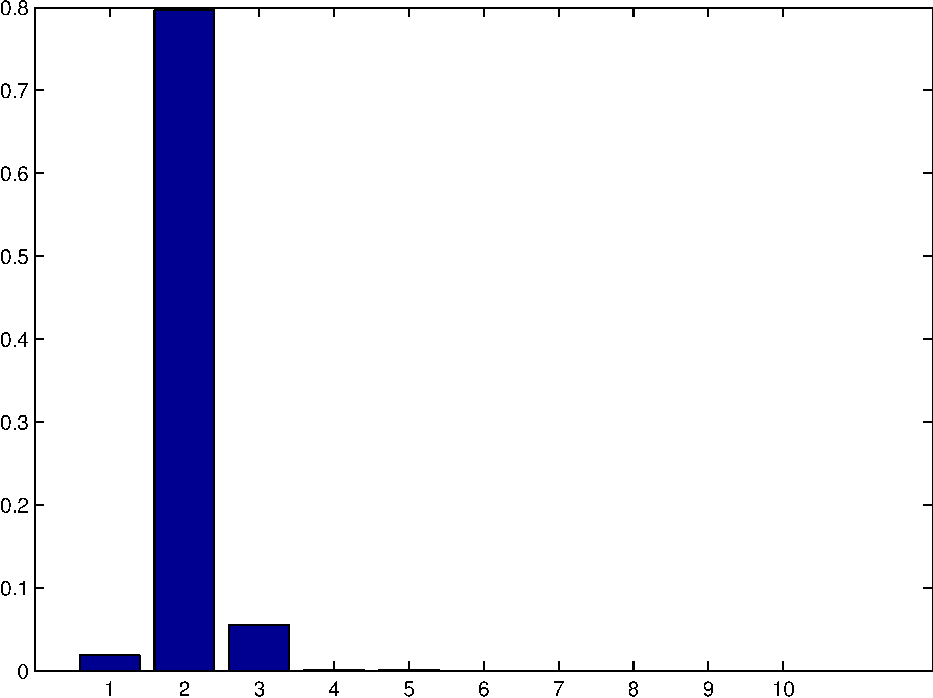
\includegraphics[width=50mm,height=42.5mm]
{../diagrams/demOilVargplvmLengthScales1}&
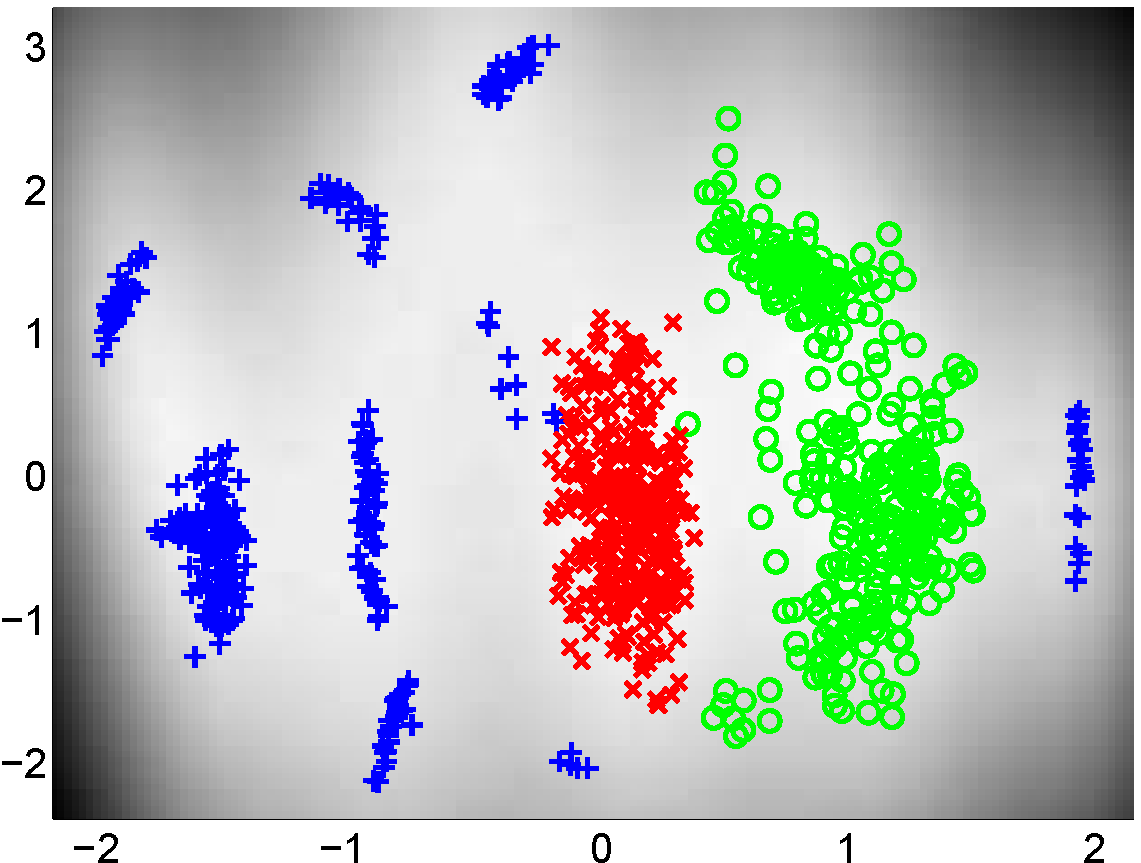
\includegraphics[width=50mm,height=42.5mm]
{../diagrams/demOilVargplvm1} &
\includegraphics[width=50mm,height=42.5mm]
{../diagrams/demOilFgplvm7.eps}\\
(a) & (b) & (c)
\end{tabular}
\caption{Panel (a) shows the inverse lengthscales found by applying the
  Bayesian GP-LVM with ARD SE kernel on the oil flow data. Panel (b)
  shows the visualization achieved by keeping the most dominant latent
  dimensions (2 and 3) which have the largest inverse lengthscale
  value. Dimension 2 is plotted on the
  $y$-axis and 3 and on the $x$-axis. Plot (c) shows the visualization found
  by standard sparse GP-LVM.
\label{fig:Oil}}
\end{center}
\end{figure*}

\vspace{-2mm}
\subsection{Frey Faces Data}
\vspace{-2mm}



\begin{figure*}[ht]
\begin{center}
\begin{tabular}{cccccccc}
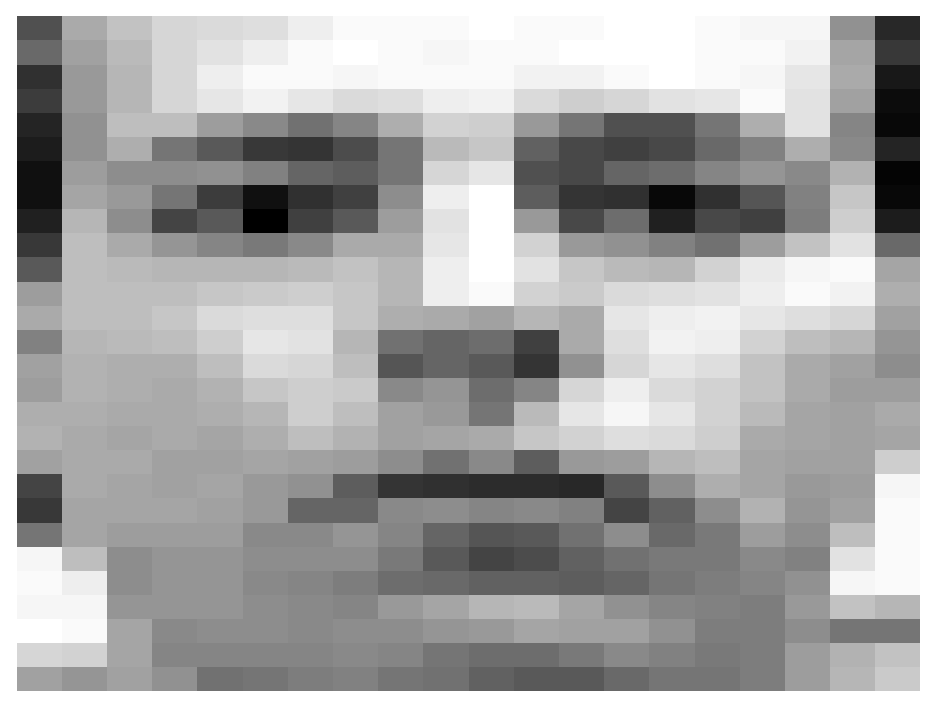
\includegraphics[width=16mm,height=13mm]
{../diagrams/demBrendanTestImag1_3.eps}&
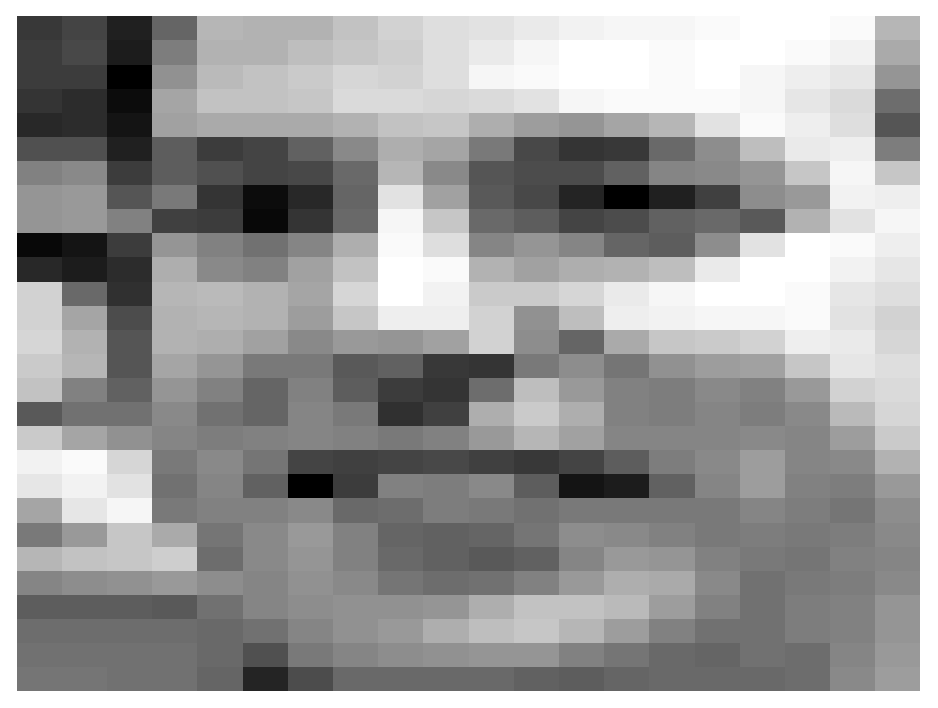
\includegraphics[width=16mm,height=13mm]
{../diagrams/demBrendanTestImag2_3.eps} &
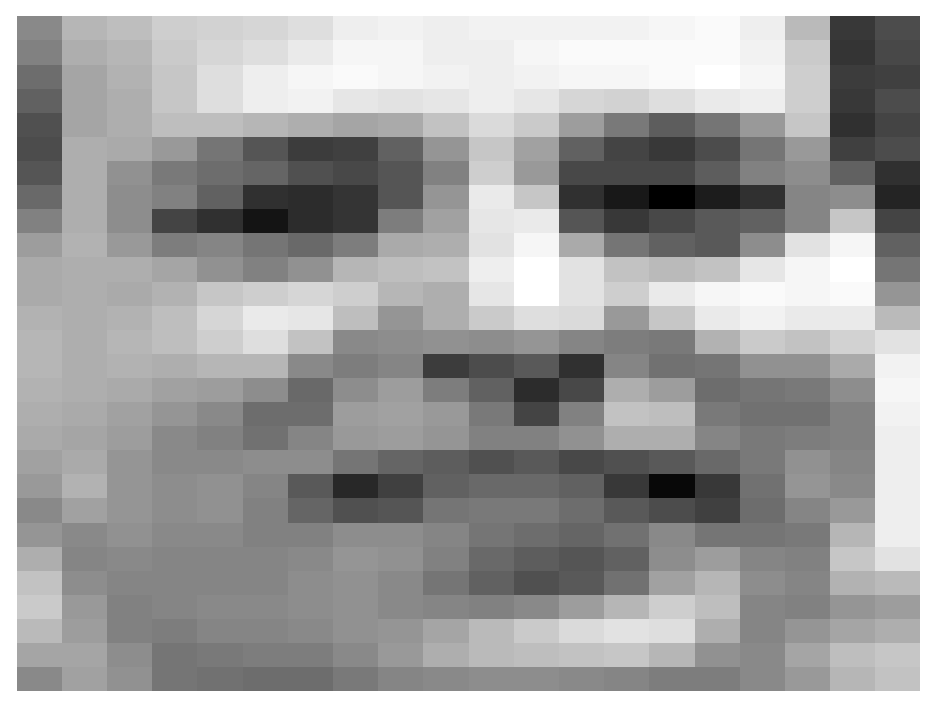
\includegraphics[width=16mm,height=13mm]
{../diagrams/demBrendanTestImag4_3.eps}&
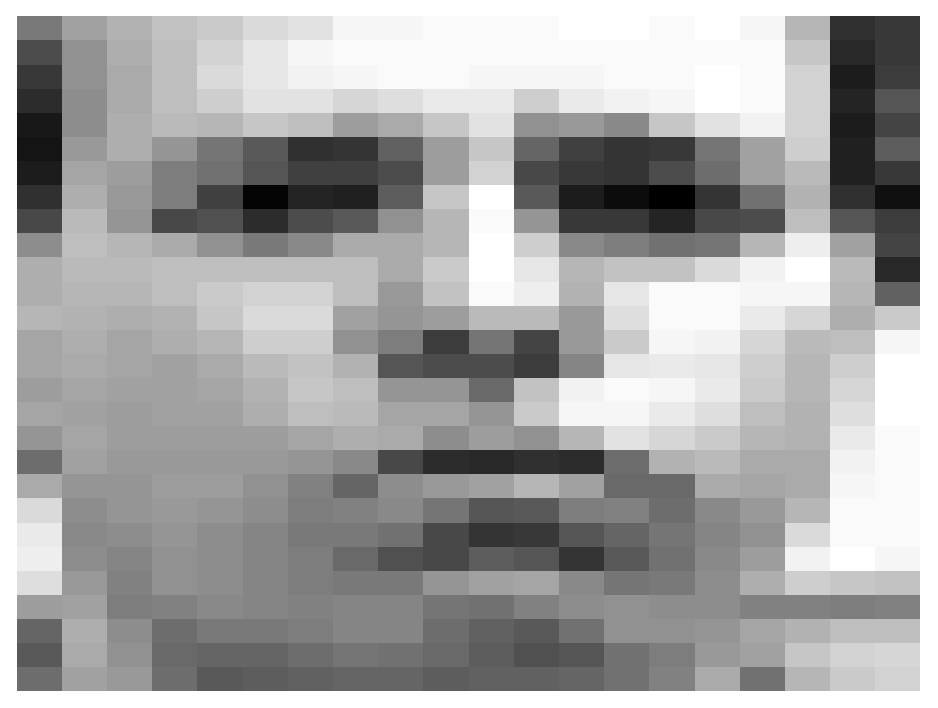
\includegraphics[width=16mm,height=13mm]
{../diagrams/demBrendanTestImag11_3.eps}&
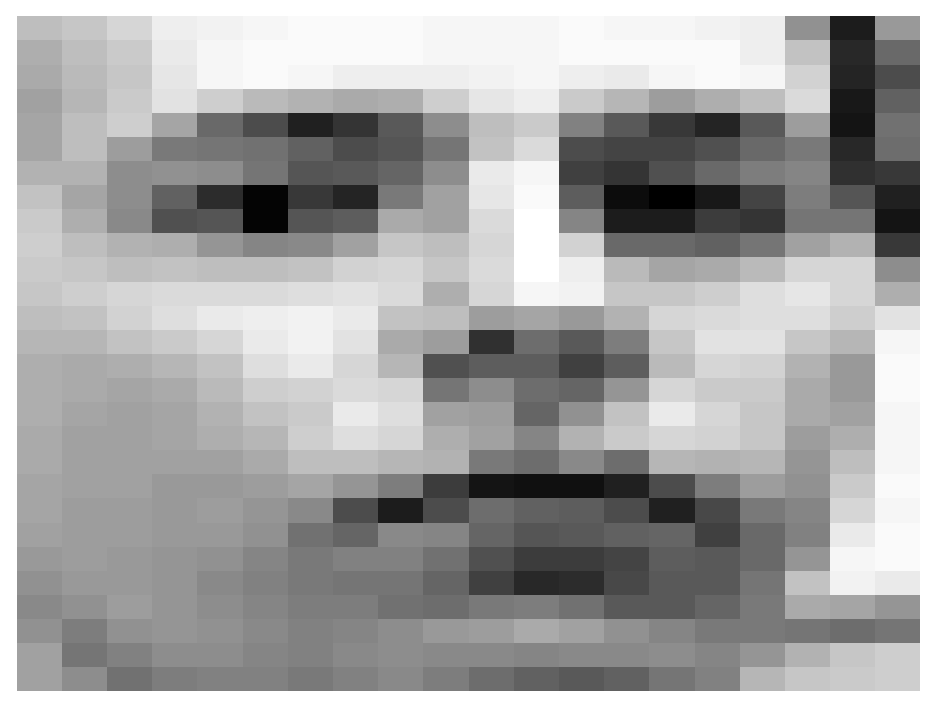
\includegraphics[width=16mm,height=13mm]
{../diagrams/demBrendanTestImag24_3.eps}&
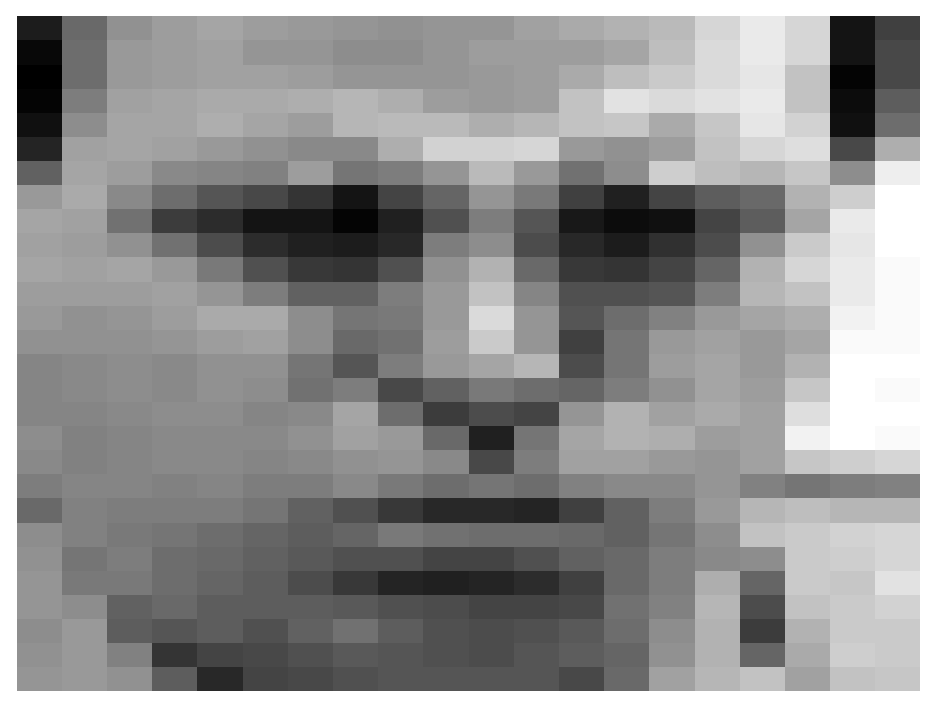
\includegraphics[width=16mm,height=13mm]
{../diagrams/demBrendanTestImag51_3.eps}&
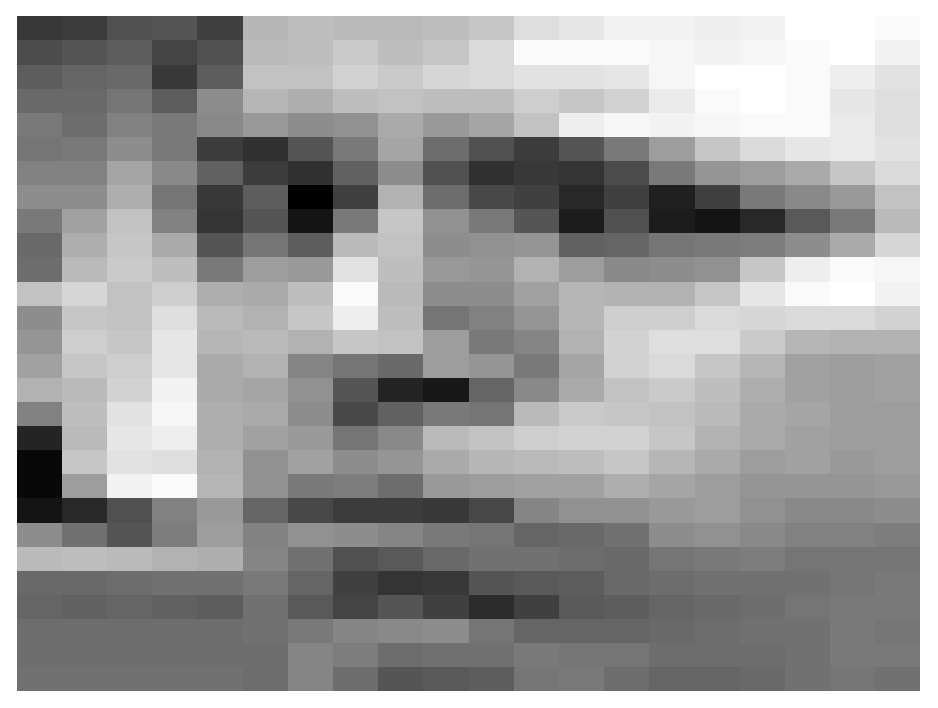
\includegraphics[width=16mm,height=13mm]
{../diagrams/demBrendanTestImag62_3.eps}&
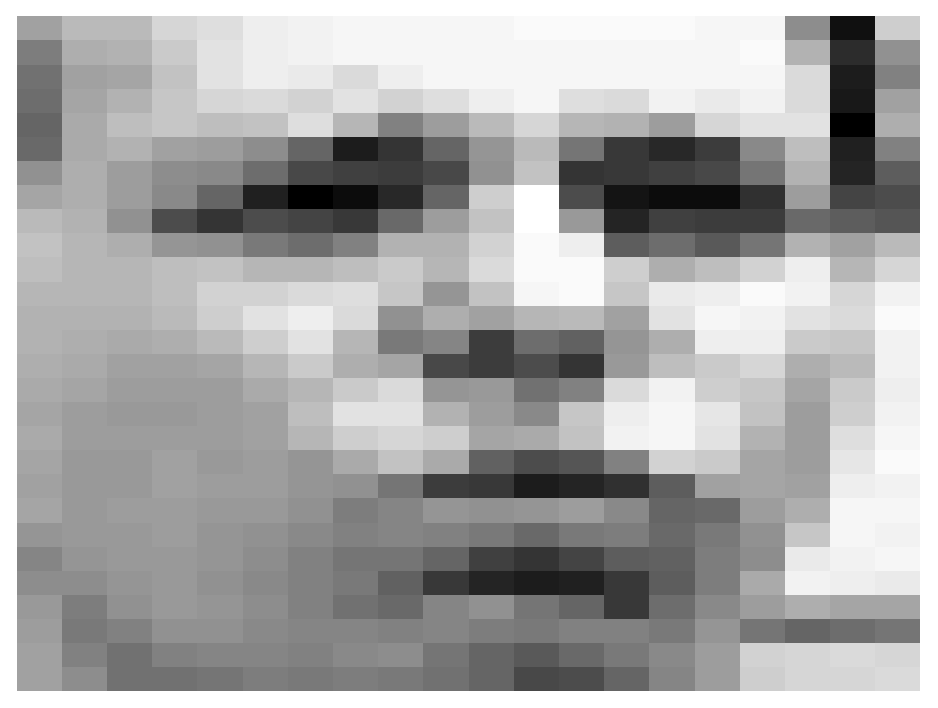
\includegraphics[width=16mm,height=13mm]
{../diagrams/demBrendanTestImag127_3.eps}\\
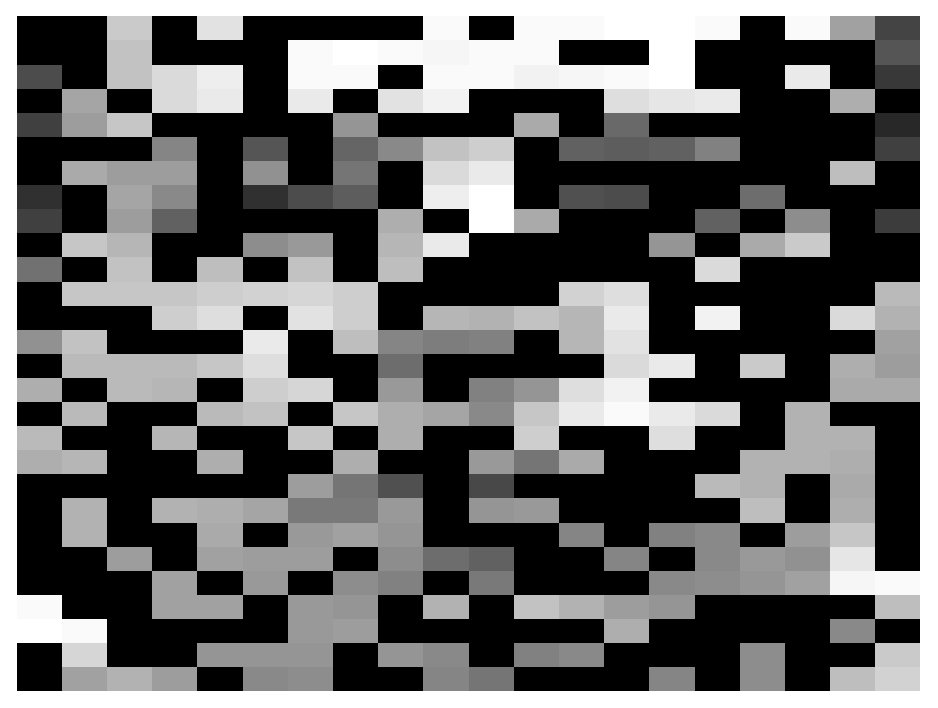
\includegraphics[width=16mm,height=13mm]
{../diagrams/demBrendanTestImag1WithMissing_3.eps}&
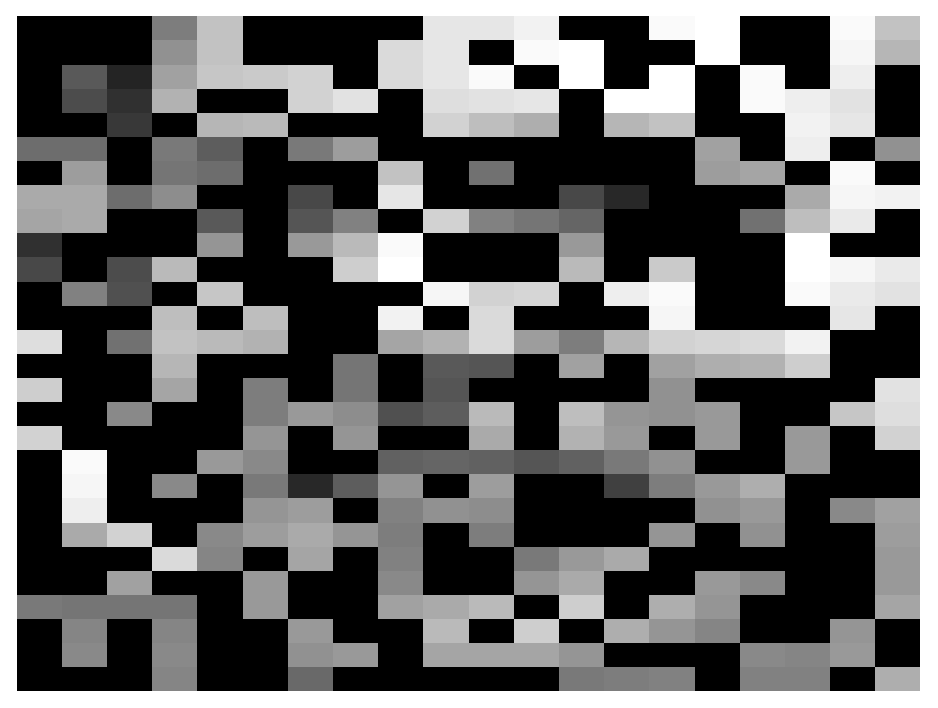
\includegraphics[width=16mm,height=13mm]
{../diagrams/demBrendanTestImag2WithMissing_3.eps} &
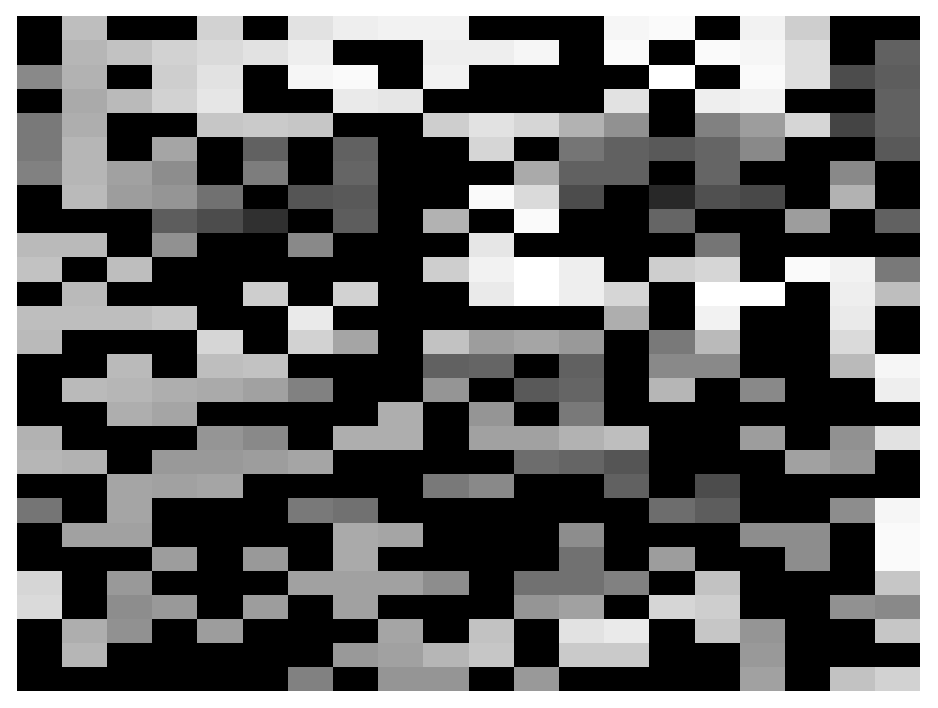
\includegraphics[width=16mm,height=13mm]
{../diagrams/demBrendanTestImag4WithMissing_3.eps}&
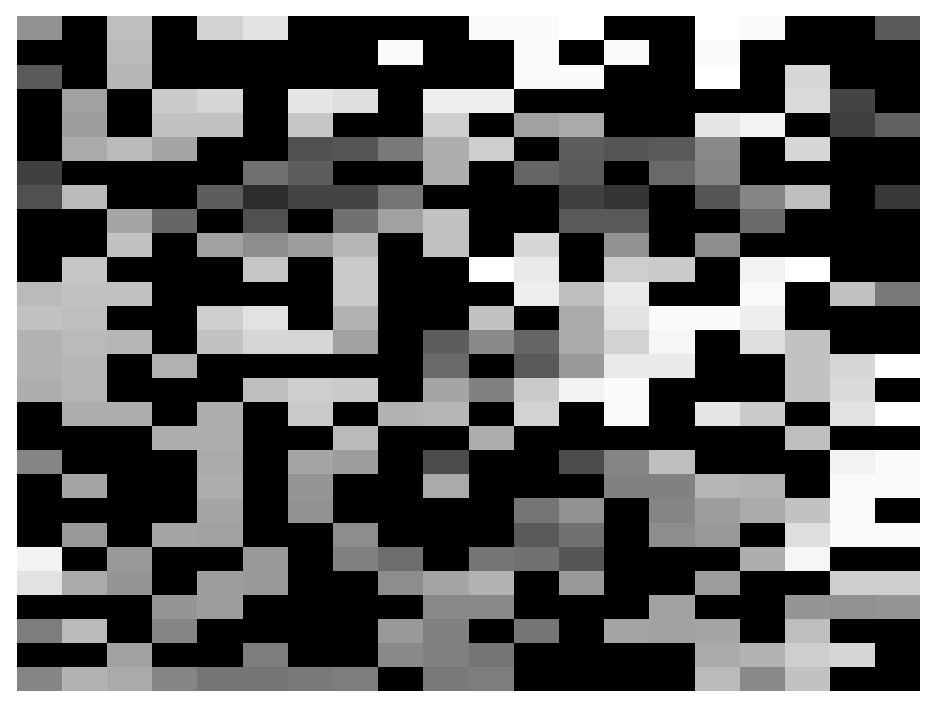
\includegraphics[width=16mm,height=13mm]
{../diagrams/demBrendanTestImag11WithMissing_3.eps}&
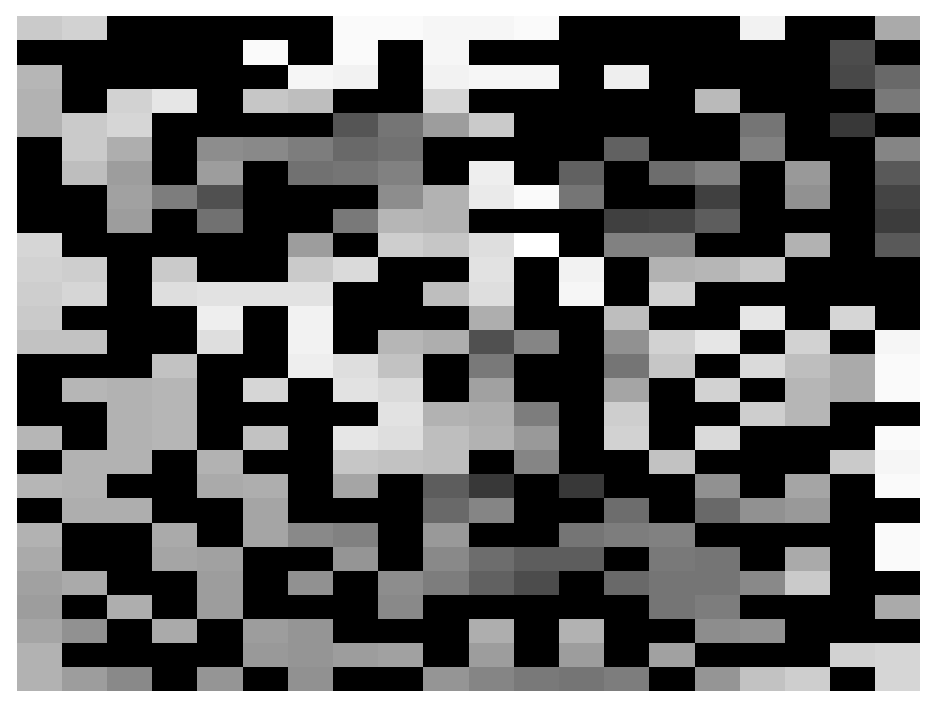
\includegraphics[width=16mm,height=13mm]
{../diagrams/demBrendanTestImag24WithMissing_3.eps}&
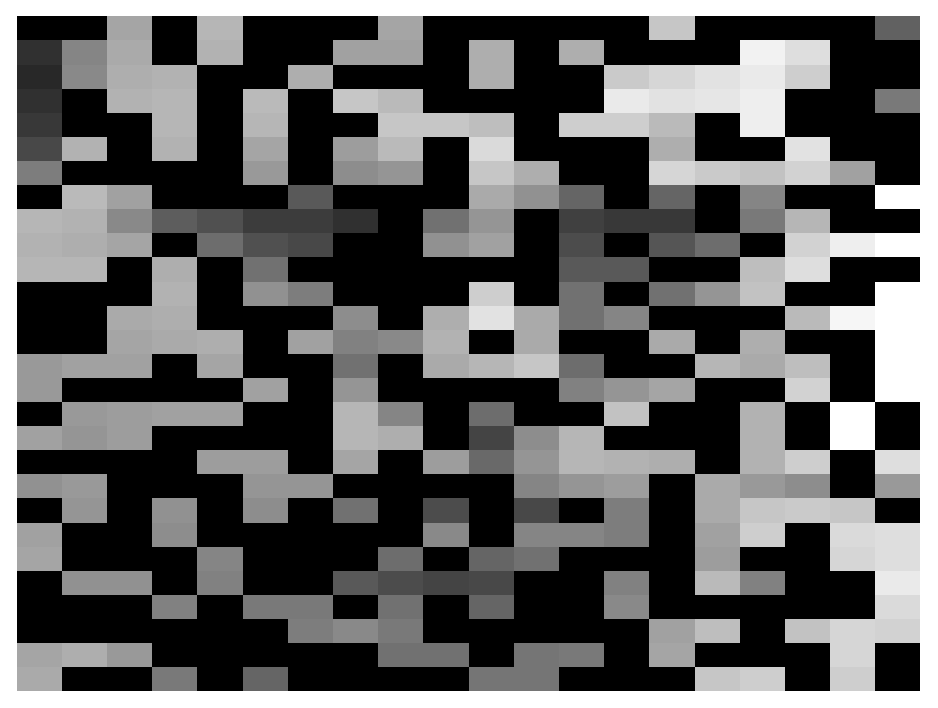
\includegraphics[width=16mm,height=13mm]
{../diagrams/demBrendanTestImag51WithMissing_3.eps}&
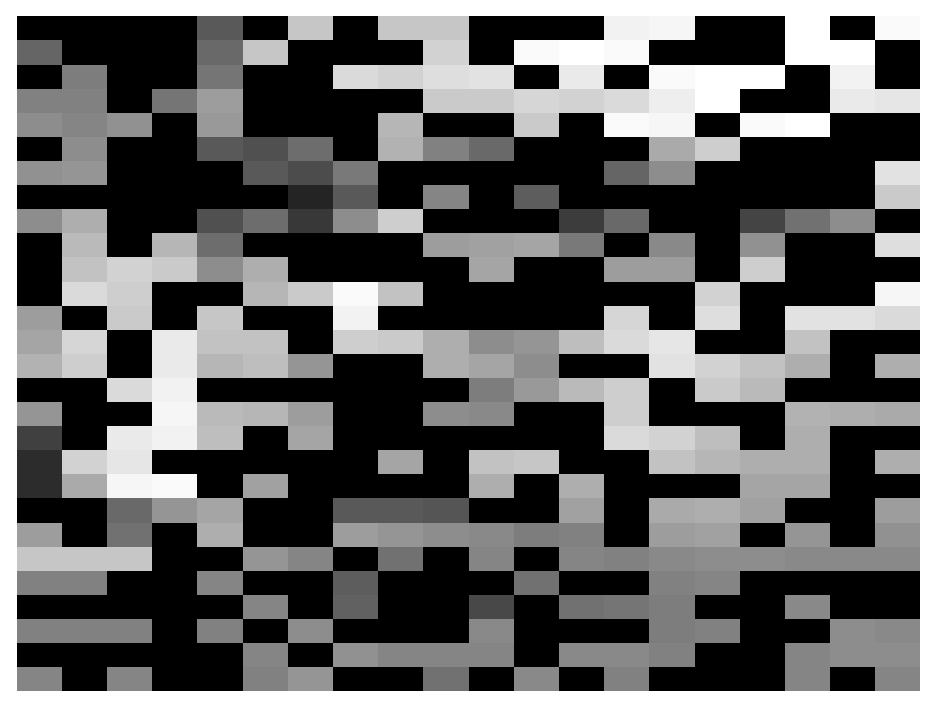
\includegraphics[width=16mm,height=13mm]
{../diagrams/demBrendanTestImag62WithMissing_3.eps}&
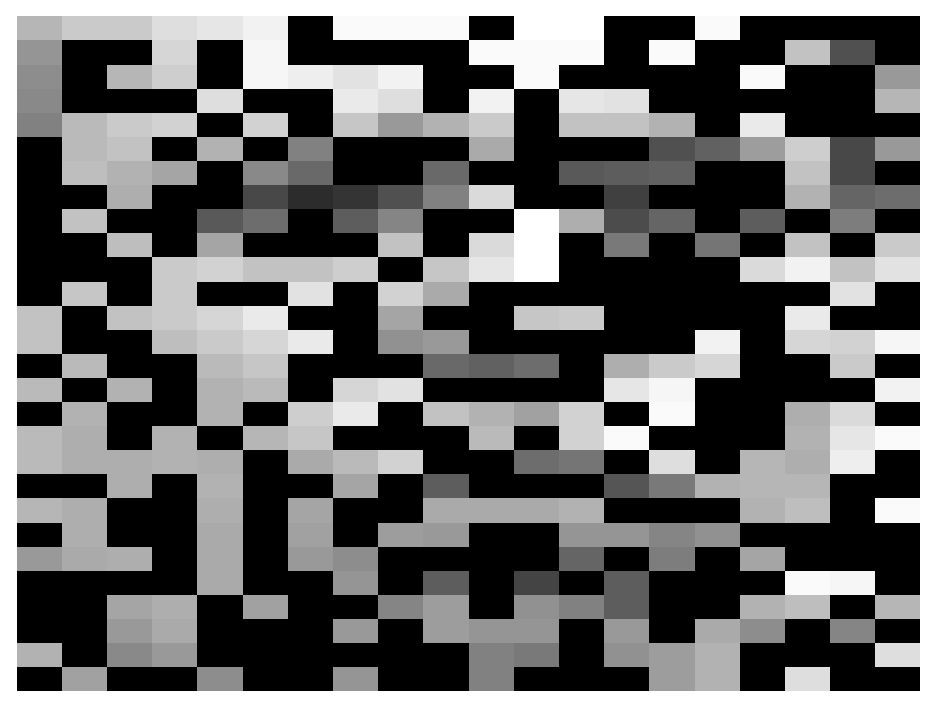
\includegraphics[width=16mm,height=13mm]
{../diagrams/demBrendanTestImag127WithMissing_3.eps}\\
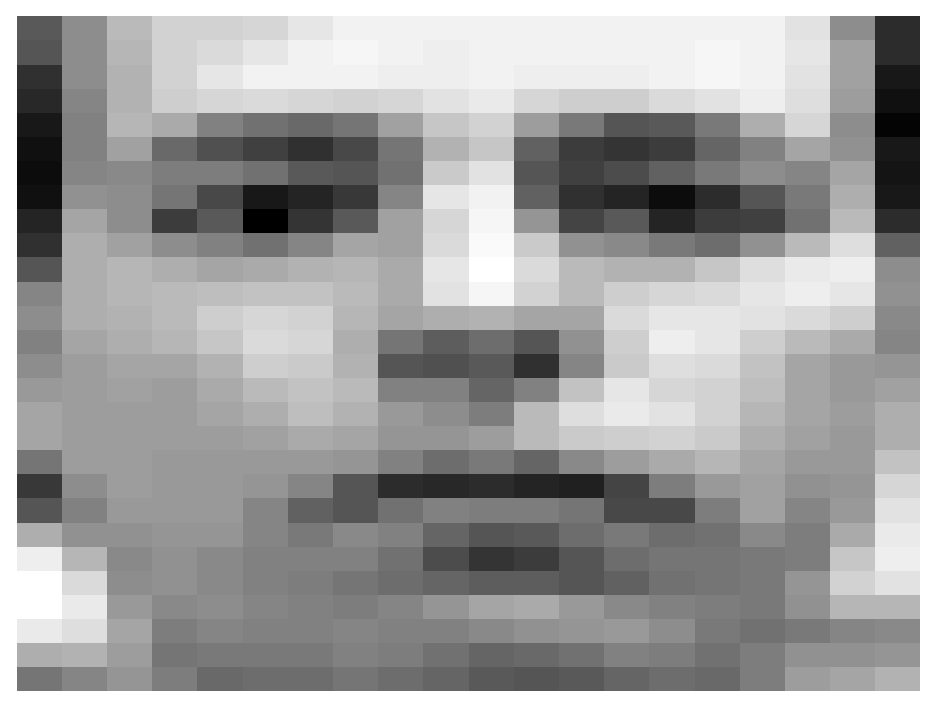
\includegraphics[width=16mm,height=13mm]
{../diagrams/demBrendanTestImag1Reconst_3.eps}&
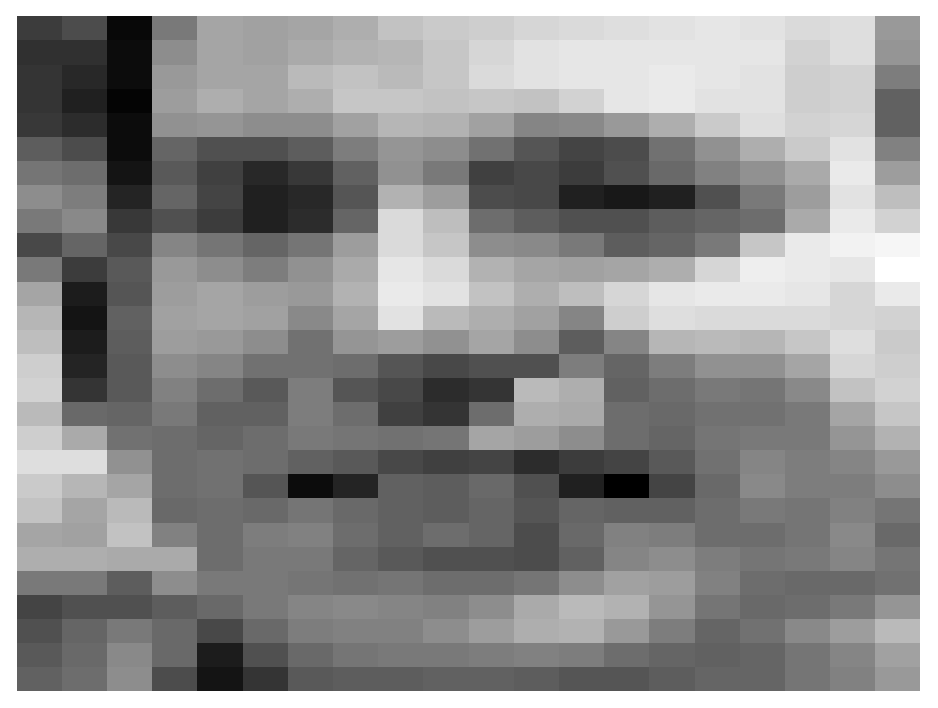
\includegraphics[width=16mm,height=13mm]
{../diagrams/demBrendanTestImag2Reconst_3.eps} &
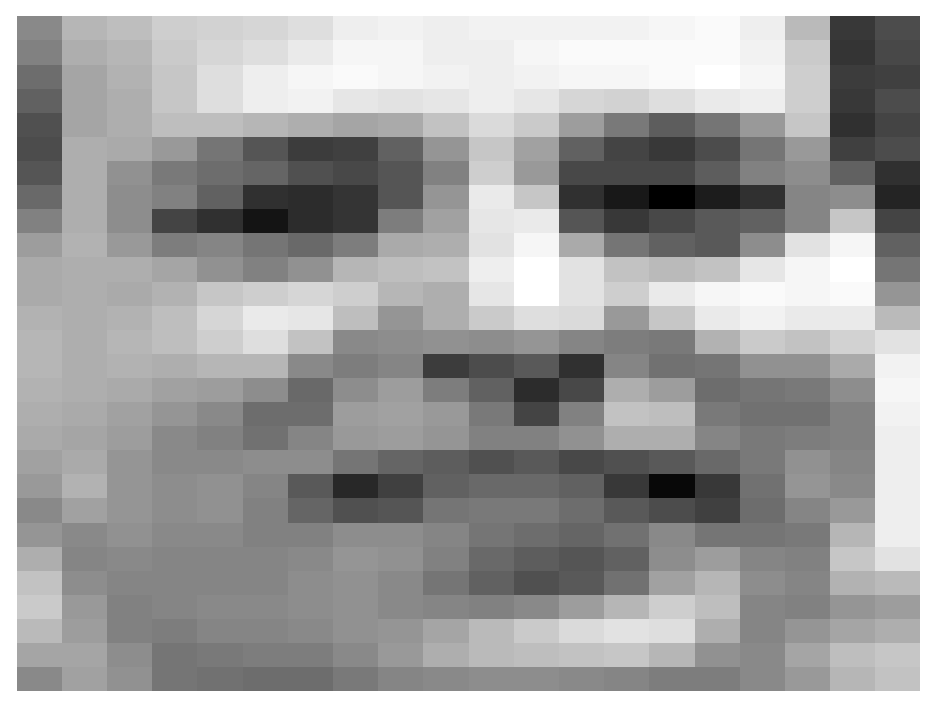
\includegraphics[width=16mm,height=13mm]
{../diagrams/demBrendanTestImag4Reconst_3.eps}&
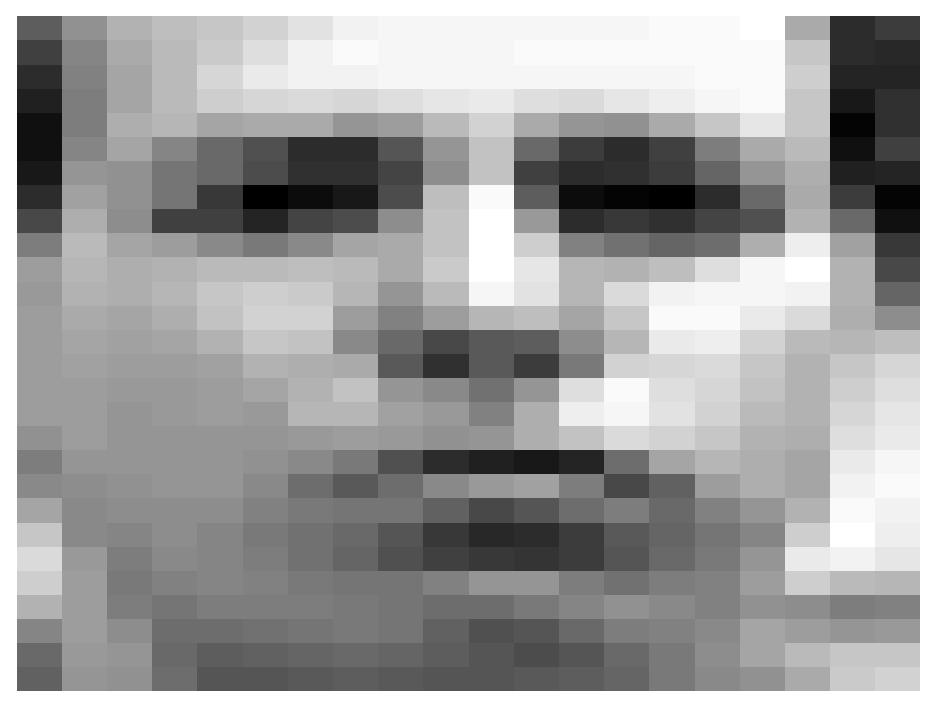
\includegraphics[width=16mm,height=13mm]
{../diagrams/demBrendanTestImag11Reconst_3.eps}&
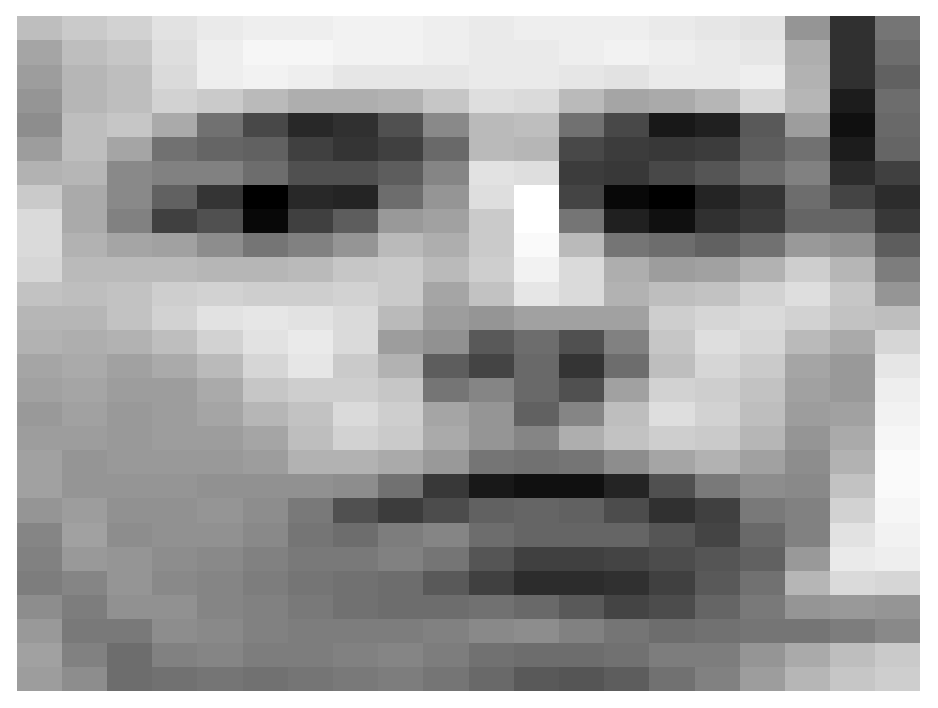
\includegraphics[width=16mm,height=13mm]
{../diagrams/demBrendanTestImag24Reconst_3.eps}&
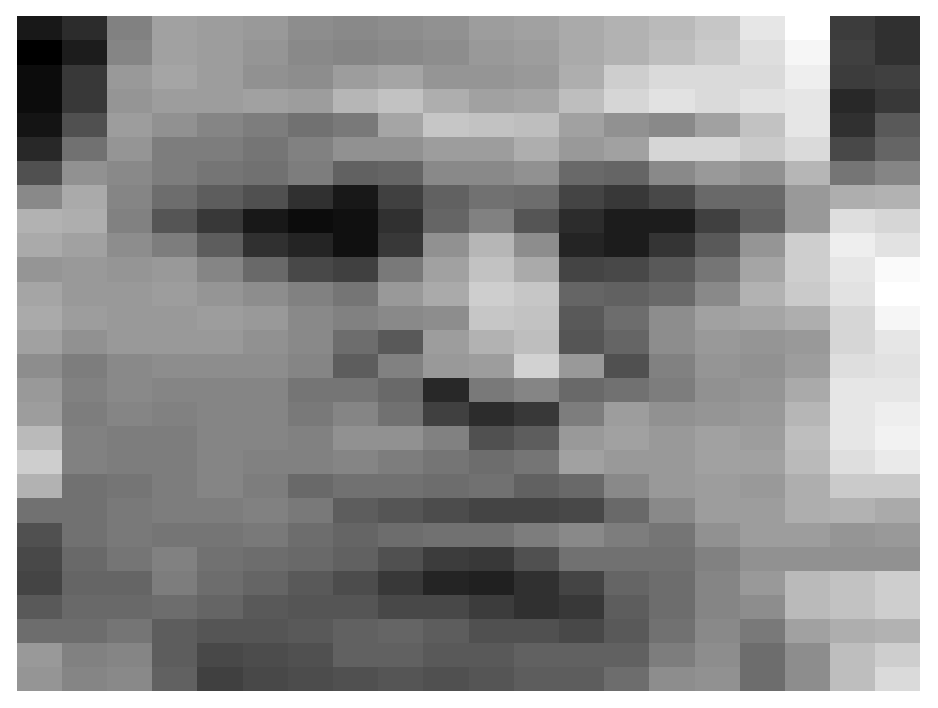
\includegraphics[width=16mm,height=13mm]
{../diagrams/demBrendanTestImag51Reconst_3.eps}&
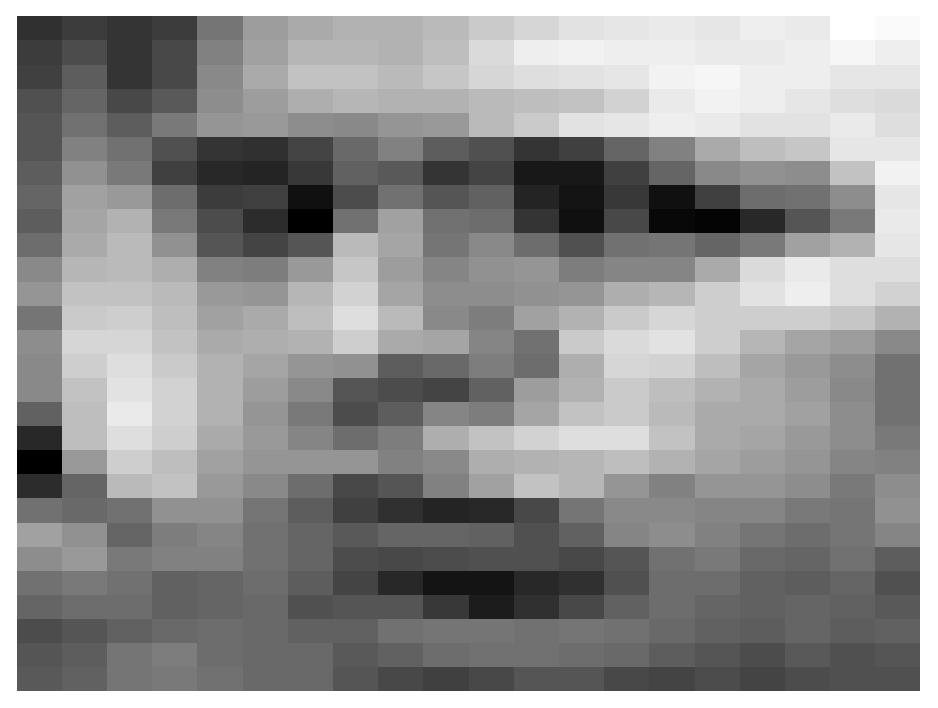
\includegraphics[width=16mm,height=13mm]
{../diagrams/demBrendanTestImag62Reconst_3.eps}&
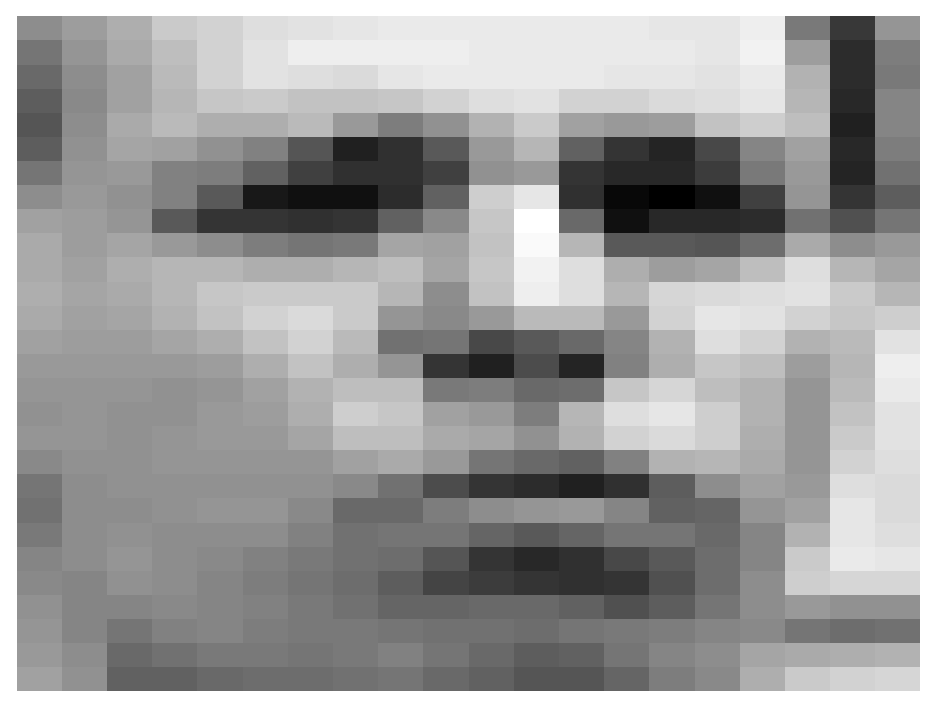
\includegraphics[width=16mm,height=13mm]
{../diagrams/demBrendanTestImag127Reconst_3.eps}
\end{tabular}
\caption{Examples of reconstruction of partially observed test images 
in Frey faces by applying the Bayesian GP-LVM. Each column corresponds to a test
image. In every column, the top panel shows the true test image, 
the middle panel the partially observed image (where missing pixels are
shown in black) and the bottom image is the reconstructed image. 
\label{fig:BrendanFaces}}
\end{center}
\end{figure*}



Here, we consider a dataset of faces \citep{Roweis:global01} taken
from a video sequence that consists of $1965$ images of size $28
\times 20$. In this dataset, we would like to exploit the ability of
the model to reconstruct partially observed test data. Therefore, we
train the model using a random selection of $1000$ images and then we
consider the remaining $965$ images as test data. Furthermore, in each
test image we assume that only half of the image pixels are
observed. The missing pixels were chosen randomly for each test
image. After training on $1000$ images, each partially observed test
image was processed separately (this involves the optimization of the
corresponding variational distribution as discussed in section
\ref{sec:predictiontest}) and the missing pixels were
predicted. Figure \ref{fig:BrendanFaces} shows a few examples of
reconstructed test images.  Each column in this figure corresponds to
a test image, where the top plot shows the true test image, the middle
one the partially observed image and the bottom image shows the
reconstructed image.  We also measure the mean absolute reconstruction
error over all test images and missing pixels and compare this error
with the standard sparse GP-LVM. This standard GP-LVM was applied
using several settings of the latent dimensionality: $Q=2,5,10$ and
$30$. The Bayesian GP-LVM was trained once using $30$ latent
dimensions. The latent variables $X$ in the standard GP-LVM and the
means of the variational distribution in Bayesian GP-LVM were
initialized through PCA.  The error for Bayesian GP-LVM was
$7.4003$. For the standard GP-LVM the error was $10.5748$, $9.7284$,
$19.6949$ and $19.6961$ for $2, 5, 10$ and $30$ latent dimensions
respectively. Notice that the standard GP-LVM has poor performance for
large value of latent dimension and achieves the best error when we
consider $5$ latent dimensions. Nevertheless, this was still worse
than the error from the Bayesian GP-LVM. Finally, Figure
\ref{fig:BrendanInverseLenghScale} shows the values of the
inverse lengthscales obtained by the maximization of the variational
lower bound. Although, in this case, the algorithm does not shrink
some of the dimensions completely to zero, it does force many of them
to obtain small values. Note that one of the dimensions (the
first from the left) seems to be the most important in
explaining the data.

\begin{figure}[ht]
\begin{center}
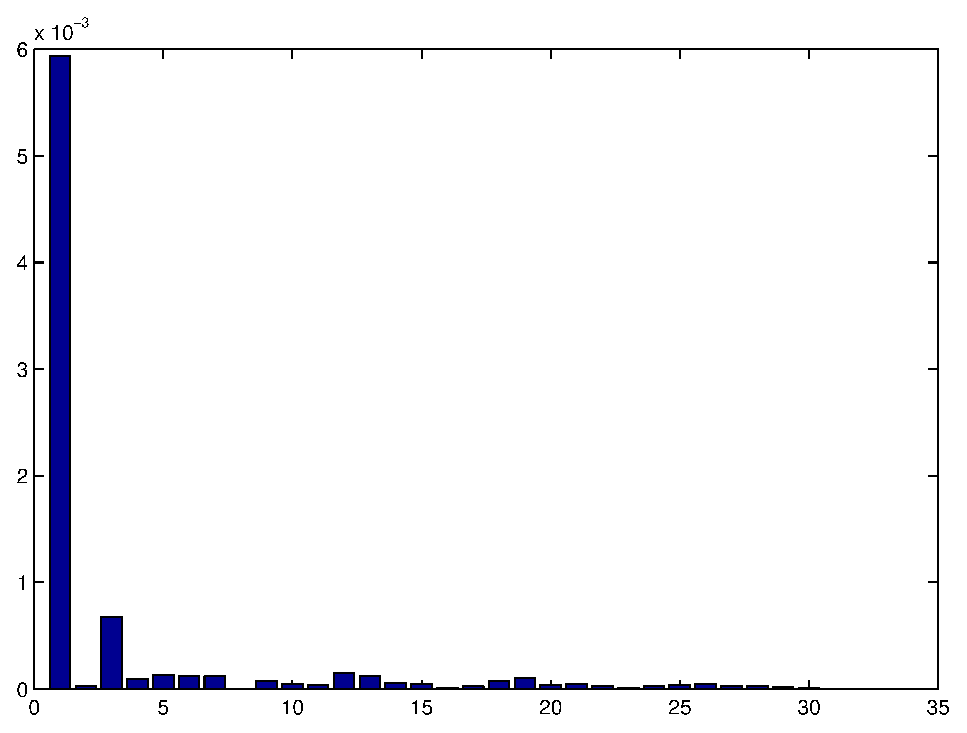
\includegraphics[width=55mm,height=45mm]
{../diagrams/demBrendanVargplvmLengthScales3.eps}
\caption{This plot shows the values of the inverse lengthscales
found by using the Bayesian GP-LVM with ARD SE kernel in Frey faces.  
\label{fig:BrendanInverseLenghScale}}
\end{center}
\end{figure}


\vspace{-6mm}
\subsection{Digits Data}
\vspace{-2mm}

In the final experiment we use the Bayesian GP-LVM to build a
generative classifier for handwritten digit recognition. We consider
the well known USPS digits dataset. This dataset consists of $16
\times 16$ images for all $10$ digits and it is divided into $7291$
training examples and $2007$ test examples.  We run $10$ Bayesian
GP-LVMs, one for each digit, on the USPS data base. We used $10$
latent dimensions and $50$ inducing variables for each model. This
allowed us to build a probabilistic generative model for each digit so
that we can compute Bayesian class conditional densities in the test
data having the form $p(\bfy_*|Y,\text{digit})$. These class
conditional densities are approximated through the ratio of lower
bounds in eq.\ (\ref{eq:ApproxpredictedDensity}) as described in
section \ref{sec:predictiontest}.  The whole approach allows us to
classify new digits by determining the class labels for test data
based on the highest class conditional density value and using a
uniform prior over class labels.  The test error made by the Bayesian
GP-LVM in the whole set of $2007$ test points was $95$ incorrectly
classified digits i.e.\ 4.73\% error. 
% This is comparable to many
%advanced discriminative classifiers that have been applied in this
%problem.

%A confusion matrix is given in Table ??. 

\vspace{-2mm}
\section{Discussion}
\vspace{-3mm}

We have introduced an approximation to the marginal likelihood of the
fully marginalized Gaussian process latent variable model. Our
approximation is in the form of a variational lower bound. With the
fully marginalized model we can automatically determine the latent
dimensionality of a given data set. We demonstrated the utility of
this rigorous lower bound on a range of disparate real world data
sets.

Our approach can immediately be applied to training Gaussian processes
with uncertain inputs where these inputs have Gaussian prior
densities. We also envisage several other extensions that
become computationally feasible using the same set of methodologies we
espouse. Dynamical models based on the GP-LVM have been proposed. It
would be straightforward to include a latent space prior with a
temporal component. This could be a Kalman filter, a general Gaussian
process \citep{Lawrence:hgplvm07} or an auto regressive Gaussian
process \citep{Wang:gpdm05}. By using our approach to propagating the
Gaussian noise through the dynamics and the latent space a variational
lower bound on the likelihood of these models could be derived. The
importance of such nonlinear models is clear from the success of
unscented Kalman filters and the related ensemble Kalman filter.

The optimization procedure has a similar computational cost to that of
previously proposed sparse GP-LVMs. We believe there is scope to
improve the speed of the optimization procedure by better exploiting
the correlation present in the parameters. A potential strategy would
be to use the control points idea used to speed up MCMC in GPs 
\citep{Titsias:efficient08} in order to encode the 
variational posterior, effectively decoupling these correlations and
speeding convergence of the optimizer.

\subsubsection*{Acknowledgements}
\vspace{-2mm}
We wish to thank Mauricio \'Alvarez for his help with the software implementation.
This work is funded by EPSRC Grant No EP/F005687/1
"Gaussian Processes for Systems Identification with
Applications in Systems Biology".

\small{
\bibliographystyle{abbrvnat}
\bibliography{lawrence,other,zbooks}
}



\end{document}
